\chapter{The Lattice Boltzmann Algorithm}
\section{General Description}
\label{implementBoltzmann}
Now that we have overviewed the pertinent concepts, we can proceed to the particulars of this implementation. As previously asserted, the heart of the Lattice-Boltzmann Algorithm lies on its discretization of the phase space\cite{franco} \cite{integerLatticeDynamics}.

To discretize the phase space, we must choose the region to simulate. In this work, we name the extremal values in the $w$ axis of the phase space $W_{min}$ and $W_{max}$.
Then, one has to fix either the size of the grid or the size of the lattice.
We name the size of the grid in the $w$ axis $N_w$ (i.e. $N_x$ or $N_{vz}$).
The size of the lattice in the $w$ axis (which we are going to name $dw$) and the extremal values are related by:
\vspace{1mm}
\begin{equation}
dw = \frac{W_{max}-W_{min} }{N_w} 
\end{equation}%\vspace{1mm}
In this work we are going to use the phase-space mass \emph{density}, which means that $\f \dd \vb{r} \dd \vb{v}$ is the density of dark matter whose position is between $\vb{r}$ and $\vb{r} + \dd \vb{r}$, and its velocity is between $\vb{v}$ and $\vb{v} + \dd \vb{v}$.
Now that we have properly defined the phase space grid, we can proceed to initialization.
For simplicity, we choose Gaussian initial conditions given by:
\begin{equation}
\f[0]= A \exp{-\frac{\vb{r}^2}{\sigma_r^2} - \frac{\vb{v}^2}{\sigma_v^2}}
\end{equation}
Where $\f[0]$ is the initialization of the phase space density, $A$ is an indirect measure of the total mass in the system, $\vb{r}$ is the vector $(x,y,z)$, $\vb{v}$ is the vector $(vx,vy,vz)$, and $\sigma_i$ are a measure of the width of the Gaussian profile in the given axis. Note that we use a single width for the spatial axes ($\sigma_{\vb{r}}$) and a single width for the velocity axes ($\sigma_{\vb{r}}$).

After initialization, the system evolves by the action of the Louville operator and the Collisional operator, nonetheless, the collisions are modeled as instant, which allows to concentrate they entire influence in a collisional step. The schematics of the algorithm can be seen easily in figure  \ref{flowchart}.

\begin{figure}[ht!]
    \centering
    %\includegraphics[width=10cm,height =7cm]{Diapositiva1.jpg}
    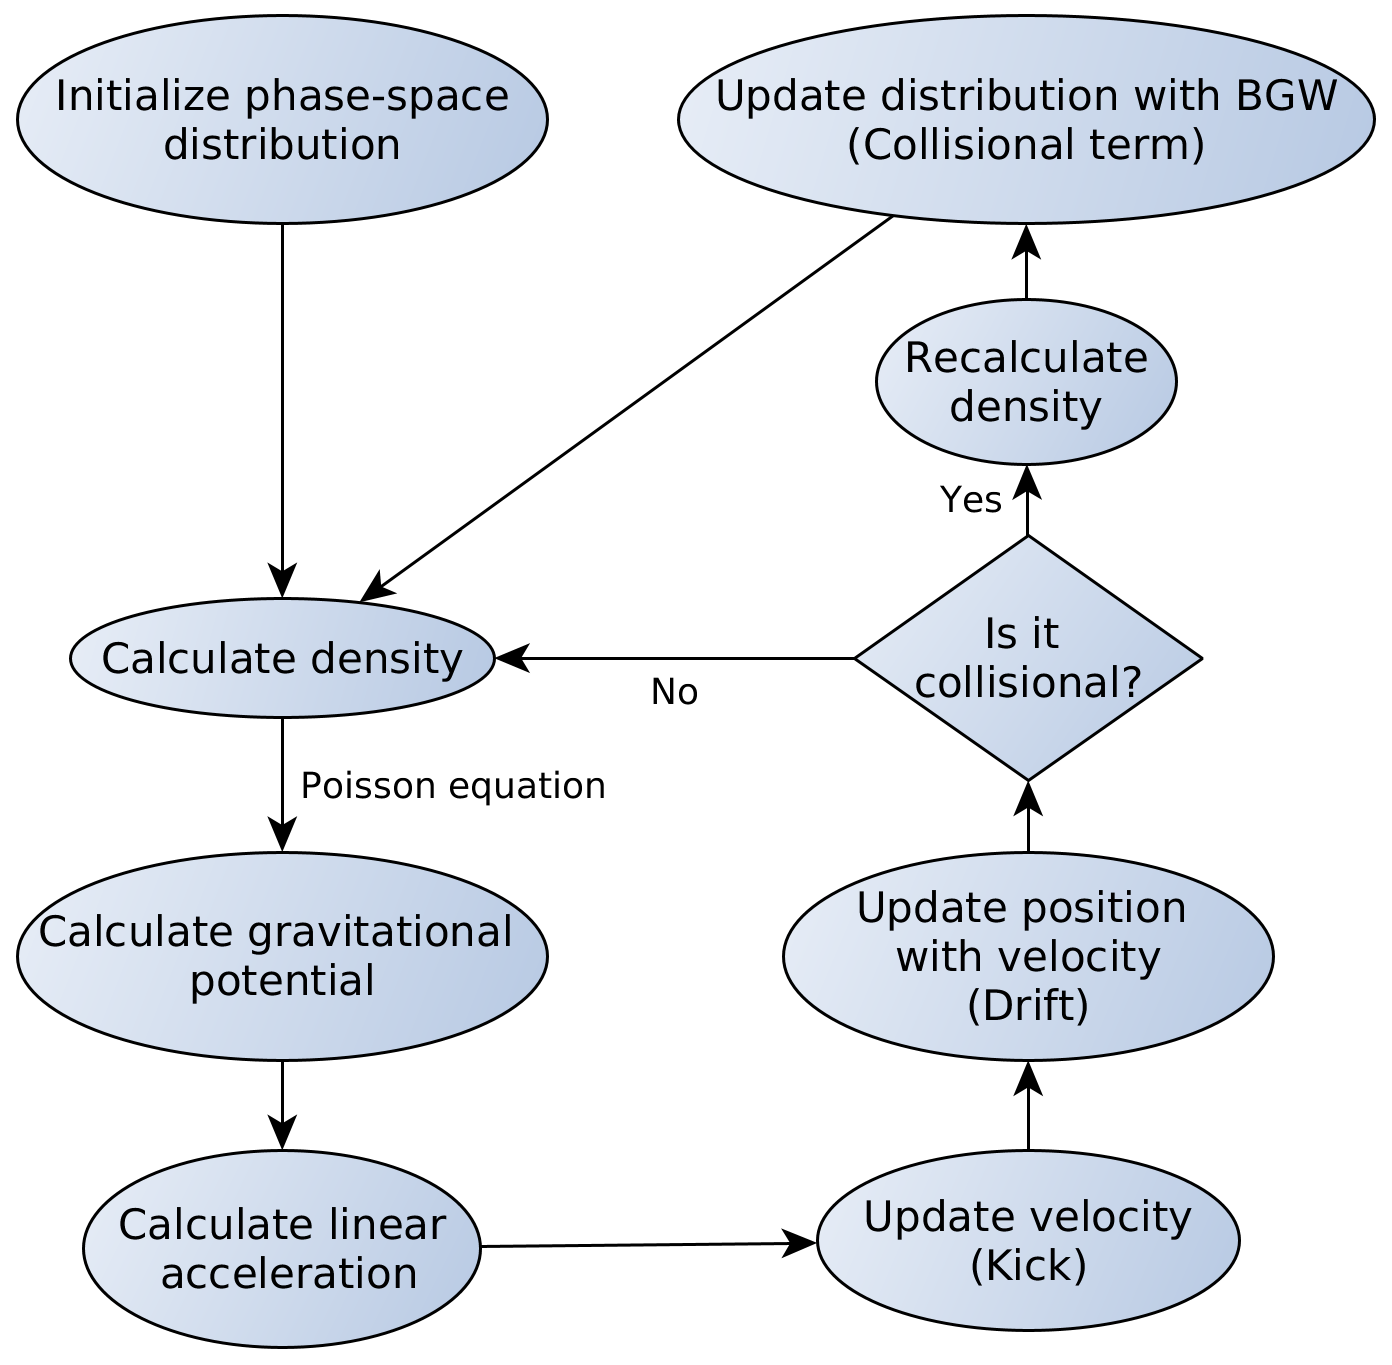
\includegraphics[scale=0.2]{imag/flowchart.png}
    \caption{Flowchat of the algorithm.}
    \label{flowchart}
\end{figure}

Now that we have defined the phase-space, we can obtain the spatial density of matter by integrating the phase space: 
\begin{equation}
\label{defDens0}
\dens[t] = \int_{-\infty}^{\infty} \! \f[t] \, \dd \vb{v}.
\end{equation}
When evaluating in the lattice the integral becomes a sum over the entire velocity lattice:
\begin{equation}
\label{defDens}
\dens[t] = \sum_{\vb{V}_{min}}^{\vb{V}_{max}} \f[t] \, \dd \vb{v}
\end{equation}
and during initialization:
\begin{equation}
\dens[0] = \sum_{\vb{V}_{min}}^{\vb{V}_{max}} \f[0] \, \dd \vb{v}
\end{equation}
Once we have calculated the density, we solve the Poisson equation to obtain the potential due to gravitational interaction:	\cite{integerLatticeDynamics}
\begin{myequation}
\laplacian \pot = 4 \pi G \dens
\end{myequation}
%TODO:añadir \\
Where $\pot$ is the gravitational potential and $G$ is the gravitational constant.
To solve the Poisson equation we use the Fourier pseudo-spectral method, which allows for very fast numerical solutions by making use of the Fast Fourier Transform algorithm. The idea is simply to apply a Fast Fourier Transform (FFT) to the density, then solve the equation in the Fourier space, and then apply an inverse transform (IFFT). In the Fourier space the Poisson equation is given by\cite{freePoisson} \cite{computerUsingParticles}
\begin{myequation}
\lambda_{\vb{k}}^2 \hat{\Phi}(\vb{k},t) = 4 \pi G \hat{\rho}(\vb{k},t)
\end{myequation}
Where $\hat{g}(\vb{k},t)$ is the Fourier transform of $g(\vb{r},t)$, and $\lambda_{\vb{k}}$ is a constant that depends on the size of the lattice and the wavevector $\vb{k}$.
$\lambda_{\vb{k}}$ is calculated according to the approximation scheme used to solve the equation.
In the the pseudo-spectral approximation, $\lambda_{\vb{k}}$ is given by:
\begin{myequation}
\lambda_{\vb{k}}^2 = \qty(\frac{2 \pi k_x}{X_{max} - X_{min}})^2 + \qty(\frac{2 \pi k_y}{Y_{max} - Y_{min}})^2 + \qty(\frac{2 \pi k_z}{Z_{max} - Z_{min}})^2
\end{myequation}
Therefore, solving the Poisson equation in the Fourier space is reduced to simple arithmetic.
Thanks to the highly efficient implementations of the Fast Fourier Transform Algorithm available nowadays, solving the Poisson equation takes very little time and computational resources.
In this work we use the Fastest Fourier Transform of the West\cite{FFTW} subroutine to handle the Fast Fourier Transforms.

Once we have calculated potential, obtaining the acceleration is straight-forward:
\begin{myequation}
\acce = -\grad \pot
\end{myequation}
Which, in the context of the lattice can be easily calculated with a central difference numerical derivative.

Now, in order to update the phase space, we must first define the time interval to simulate: we name $N_t$ the number of time \emph{instants} to simulate and $\dd t$ the length of each of such instants.
After calculating the acceleration and defining $\dd t$, we can update our phase space.
As mentioned in section \ref{boltz}, the subtlety here is that we will only use integer arithmetic, which means that we do not exactly care about the change in velocity during a time $\dd t$ but for how many cells in the phase space lattice that change represents. This is modeled by:
\begin{equation}
\vb{v}_{n+1} = \vb{v}_n + \toInt{\vb{a}_n \dd t}
\end{equation}%\\%\vspace{5mm}\\
With $\toInt{x}$ representing the operator \tqt{to nearest integer}, so that $\vb{v}$ and $\toInt{\vb{a} \dd t}$ are vectors of integers and $n$ represents the time instant. The update of the velocity is known as \tqt{kick}. Analogously, the update of the position is known as \tqt{drift}, and is given by:
\begin{myequation}
\vb{r}_{n+1} = \vb{r}_n + \toInt{\vb{v}_n \dd t}
\end{myequation}\\
The use of only integer arithmetics allows for the elimination of the rounding error but introduces lattice noise. Regardless, this method creates a one to one map with the continous solution\cite{franco} \cite{integerLatticeDynamics}.\\ \\ 
\vspace{-1mm} The \tqt{kick} and \tqt{drift} together are known as the \tqt{Streaming} step, and it represents the classical movement of particles under a potential but without considering the collision of particles. 
If we want a collisionless simulation, we can just calculate again the density and continue the algorithm from there. If we want a collisional simulation, we must define a collisional step.

\section{The Collisional Step}
As previously mentioned, solving the collisional integral $C[f]$ is not straight-forward, as it depends on the modeling of the short range interactions that we decide to assign to the dark matter particle.
Given that the short range interaction of dark matter is unknown, we avoid using an specific description of the microscopic interactions and choose to use a mesoscopic approach instead, as discussed in section \ref{bgk}. The BGK collisional operator is given by:
\begin{equation}
C[f] = -\frac{1}{\tau}(\f - f_e(\rv))
\end{equation}
Which in the context of the direct integration scheme used in the simulation becomes:
\begin{equation}
f(\vb{r} + \vb{v} \dd t,\vb{v},t) = \f - \frac{\dd t}{\tau}(\f - f_e(\rv))
\end{equation}\\
The idea behind this approach is to recover the macroscopic description of the fluid without committing to a particular microscopic description. In this scenario, the macroscopic effects of the collisions is a local relaxation towards equilibrium, which the BKG operator models using a relaxation time $\tau$ and a local equilibrium distribution $f_e(\rv)$. 

In order to implement a collisional operator we add a collisional step after the streaming step, in which the system performs a relaxation with characteristic (relaxation) time $\tau$ towards the local equilibrium distribution $f_e(\rv)$. 
It is important to notice that the BGK collisional operator is a \emph{scattering} operator and does not consider annihilation or creation of particles. 

After defining the collisional term, we have to choose a distribution function $f_e(\rv)$. We claim that the phase space distribution relaxes towards equilibrium, which means a displacement in the phase space and not the introduction or annihilation of mass.
Therefore, the equilibrium distribution must be perfectly \emph{normalized}  in order to enforce particle number conservation. We normalize this equilibrium distribution by using macroscopic quantities obtained by integrating the velocity part of the phase space.
This macroscopic quantities are: the volumetric density $\dens$, the macroscopic velocity $\vb{u}(\rv)$ and the internal energy $e(\rv)$.

The volumetric density is the same density we have been using so far defined by the integral of equation \ref{defDens0}. The macroscopic velocity $\vb{u}(\rv)$ is defined by the integral:
\begin{equation}
\vb{u}(\rv) = \int_{-\infty}^{\infty} \! \f[t] \, \vb{v}  \dd \vb{v}.
\end{equation}

When evaluating in the lattice the integral becomes:
\begin{equation}
\label{defVel0}
\vb{u} = \sum_{\vb{V}_{min}}^{\vb{V}_{max}} \f[t] \,  \vb{v} \dd \vb{v}
\end{equation}
And the internal energy is defined by the integral:
\begin{equation}
e(\rv) = \frac{1}{2} \int_{-\infty}^{\infty} \! \f[t] \, (\vb{v} -\vb{u})^2 \dd \vb{v}.
\end{equation}
Which also becomes a sum when evaluating in the lattice:
\begin{equation}
\label{defEn0}
e(\rv) = \frac{1}{2} \sum_{\vb{V}_{min}}^{\vb{V}_{max}} \f[t] \,  (\vb{v} -\vb{u})^2 \dd \vb{v}
\end{equation}\vspace{2mm} 

Note that we are not including explicitly the mass of the dark matter particle in this integrals because it has already been included in the phase space definition.

Now that we have well defined macroscopic variables, we can proceed to choose an equilibrium distribution. Such distribution must obey the next condition:
\begin{equation}
C[f_e] = 0
\end{equation}
Which simply means that if the system is already in local equilibrium, then there is no relaxation. This condition can also be stated as \tqt{the equilibrium function must be a collisional invariant}. In order for $f_e(\rv)$ to be a collisional invariant, it must be build with variables that are also collisional invariant. Fortunately, the macroscopic variables already defined in this chapter are also collisional invariants, and so, we can use them to build equilibrium distributions. The idea behind normalization is to obtain the same macroscopic variables when integrating over $f_e(\rv)$ instead of $\f$.  In this work we use distributions based on the Maxwell-Boltzmann velocity distribution. Alternative equilibrium distributions functions can be considered and may be of interest, but they are beyond the scope of this work. In particular, quantum Maxwellians may be used to include annihilation and creation of particles, and the effects of Bose-Einstein, Fermi-Dirac statistics\cite{2010arXiv1009.3352F}.

The equilibrium function to use is a classical Maxwellian properly normalized for the case of interest:
\begin{equation}
f_e(\rv) = \frac{\rho}{[2 \pi \ e(\rv) ]^{D/2}} \exp[-\frac{(\vb{v}-\vb{u})^2}{2 \ e(\rv)}]
\end{equation}
Where $D$ is the number of spatial dimensions. For example, if the system is a three dimensional dark matter halo, then D will be equal to three.
The Maxwell distribution was originally used to describe the probability distribution of the velocity in a gas under kinetic theory assumptions. Here, we assume collisions as a phenomena that happens instantly, and during the time in between, the mechanics of the system is governed by the self-gravitational potential. Therefore, the Maxwell distribution is a good starting point for the collisional equilibrium distribution.


\subsection{Units on the simulation}

To set the units we fix the value of one spatial unit ($us$), one unit of time ($ut$), and one unit of mass ($um$) of the simulation, and from there, we proceed to calculate the values of the physical constants in our units.
The physical constant of interest here is the gravitational constant, since it gives the coupling of the gravitational interaction.
We chose units to simulate a dark matter halo of dimensions akin to the Milky Way's dark matter halo. Because of stability conditions, the units may differ between runs, therefore, they are specified at the beginning of each section in the results chapter.

\chapter{Results}
For the development of this work we wrote and ran three simulations: a  two dimensional phase space simulation (one spatial and one velocity dimension), a four dimensional phase space simulation, and a six dimensional phase space simulation. 
The first one was develop in order to reproduce the results of Philip Mocz and Sauro Succi published in 2016 \cite{integerLatticeDynamics}, and the results of Sebastian Franco published in 2017 \cite{franco}.
In addition to reproducing results, we also extended the simulation to account for a collisional operator and tested it with different initial conditions.

The four dimensional simulation was develop as a step to develop the six dimensional simulation. Developing a four dimensional simulation allows to implement and test the specifics of increasing dimensionality without much of the visualization problems that arise from a six dimensional simulation. 

The six dimensional simulation is one of the main scopes of this work. The simulation was implemented successfully, however, due to the high RAM memory requirements of the Lattice-Boltzmann method, the resolution is heavily constrained. Even using the HPC cluster avalible at \tqt{Universidad de los Andes}, the resolution of the simulation was too poor to reproduce the results from the other two simulations.

\section{The two dimensional phase space}
%\vspace{-5mm} \vspace{1mm} %descomentar

For the two dimensional simulation we only need two axes, which allows for a very high resolution in the simulation. We used an squared grid characterized by:
\begin{align}
W_{min} &= -1\\
W_{max} &= 1\\
N_w &= 2048\\
dw &= 1/1024
\end{align}
As mentioned in section \ref{implementBoltzmann}, $W$ represents the axis (in this case $r$ or $v$), $N_w$ represents the size of the grid in the $w$ axis, $dw$ represents the size of a lattice unit in the $w$ axis and $-1$ and $1$ are the extremal values of the phase space in the $w$ axis.
We always use grid sizes of the form $N_w = 2^n$ with $n$ positive integer, because the Fast Fourier Transform algorithm performs better and faster when calculating discrete transforms of sizes $2^n \ 3^m \ 5^l$ for n,m,l positive integers.%\\ \\ 
%\vspace{-1mm}

In this section we are going to use three initial conditions:
\begin{itemize}
\item A Gaussian density profile used to test the code, and explain the expected behaviors of the phase space density time-evolution.
\item A Jeans instability test, in which we reproduce the spatial conditions for a jeans stability and use a Gaussian profile for the velocity distribution. These conditions are used to reproduce the previous work aforementioned.
\item A Bullet Cluster-like initial conditions, in which we have two Gaussian profiles (each one with its own variance and amplitude) separated by a given distance. One of the main scopes of this work is to analyze the Bullet Cluster-like system and compare the phase space evolution of the collisional case its collisionless counterpart.
\end{itemize}
\subsection{No collisional case}
We begin with the Gaussian conditions because of their simplicity and ease to analyze.
The initialization of the phase space can be seen in figure \ref{1dInit}, along with its correspondent spatial density.
It is easily observed that the density profiles are Gaussian distributions.
After initialization we proceed to calculate the potential and the acceleration, which can be seen in figure \ref{1dInit2}.
The values used to initialize the phase space were:
\begin{align}
\sigma_r &= 0.2 \ \text{us} \\
\sigma_v &= 0.2 \ \text{us} / \text{ut} \\
A &= 50  \ \text{um}
\end{align} %TODO actualizar valores de simulacion, incluida masa total
Which yields a total mass of $1.26\e{12}$ M$_{\odot}$, a value in accordance with recent estimates of the total mass of our galaxy's dark matter halo \cite{2013JCAP07016N}. %TODO colocar la verdadera masa y unidades.

\begin{figure}[h!]
    \centering
    %\includegraphics[width=10cm,height =7cm]{Diapositiva1.jpg}
    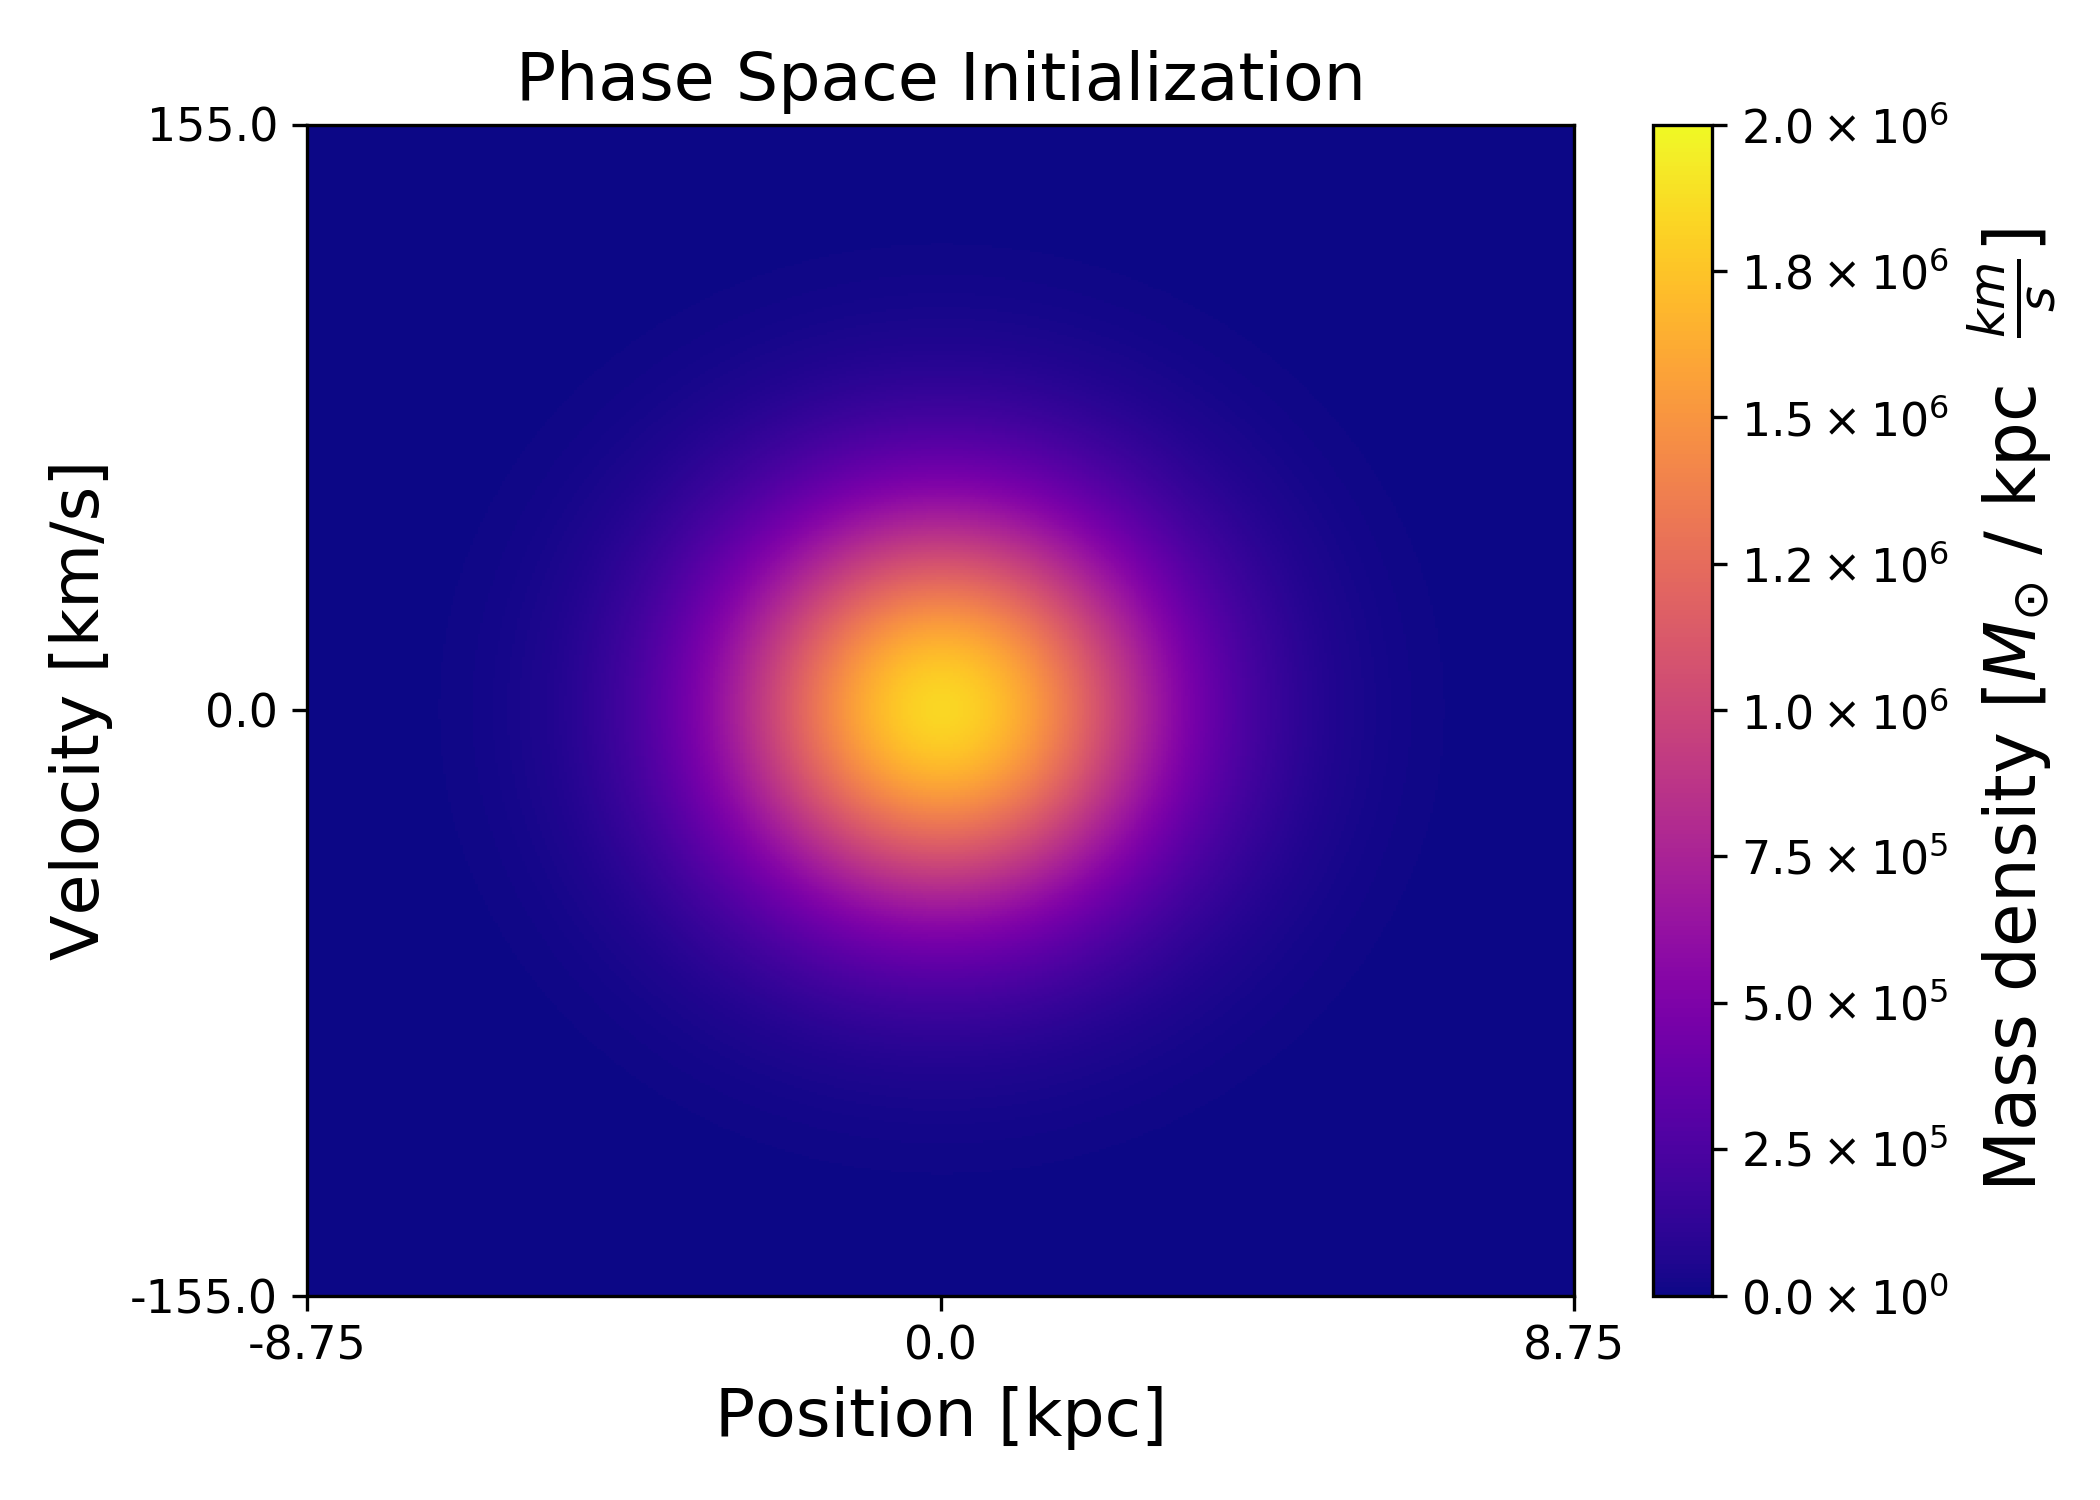
\includegraphics[scale=0.6]{imag/1dInitPS.png}
    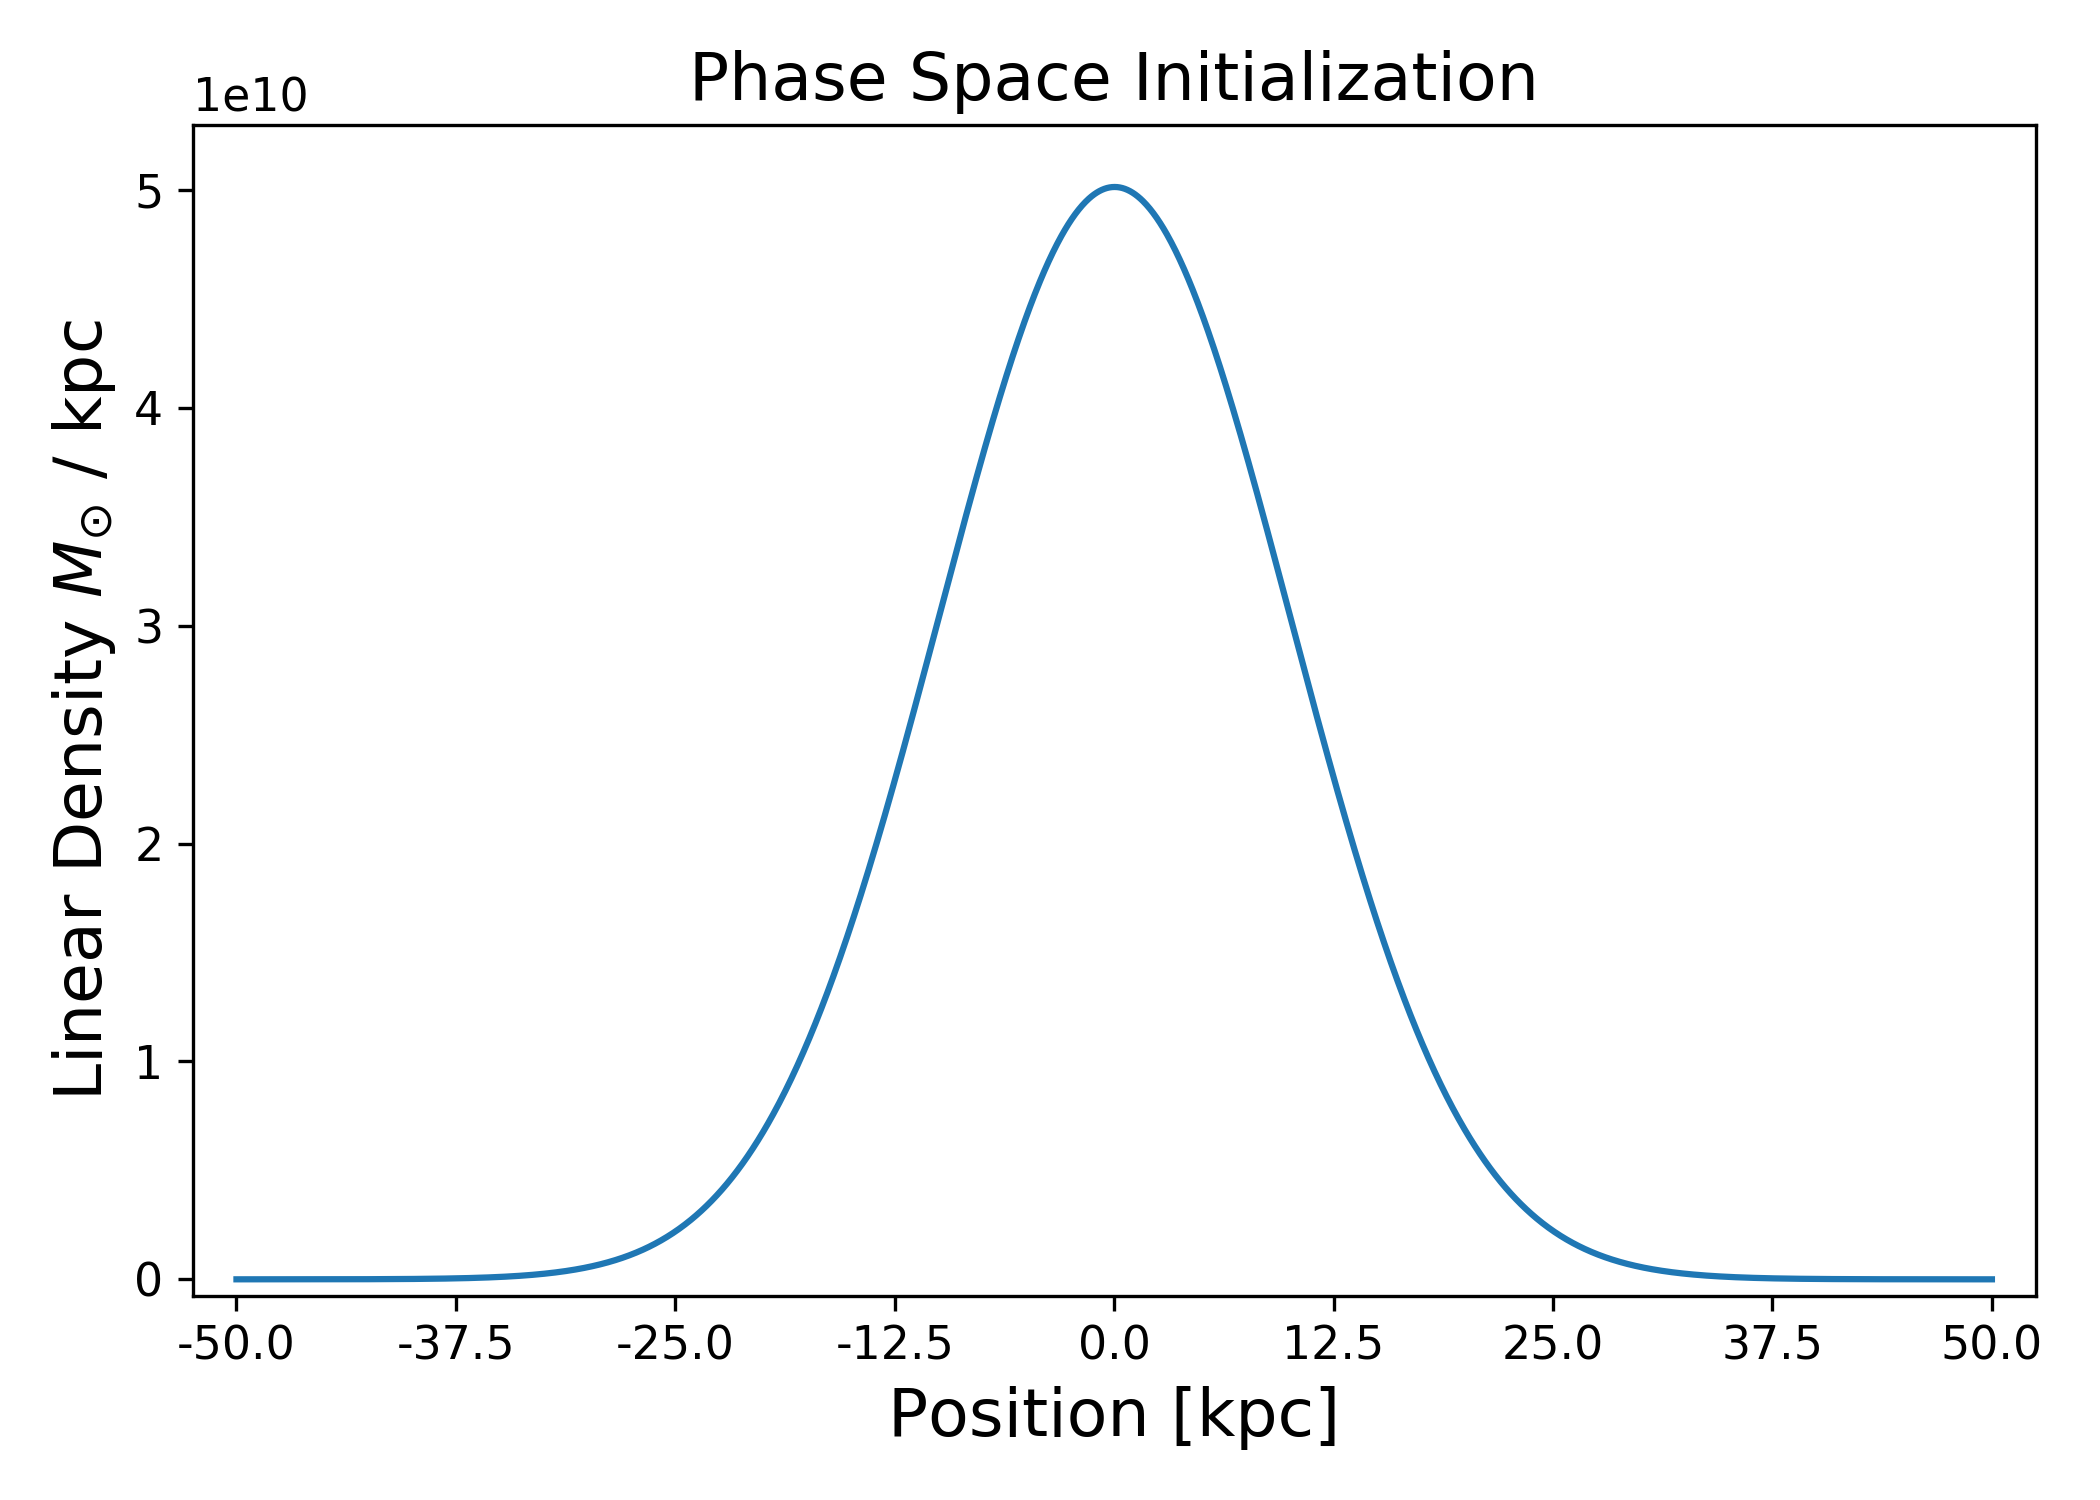
\includegraphics[scale=0.6]{imag/1dInitDens.png}
    \caption{Up: initialization of the phase space. Position is represented in the $x$ axis, and velocity in the $y$ axis of the plot. Down: the spatial density obtained through integration. }
    \label{1dInit}
\end{figure}
\newpage
\begin{figure}[h!]
    \centering
    %\includegraphics[width=10cm,height =7cm]{Diapositiva1.jpg}
    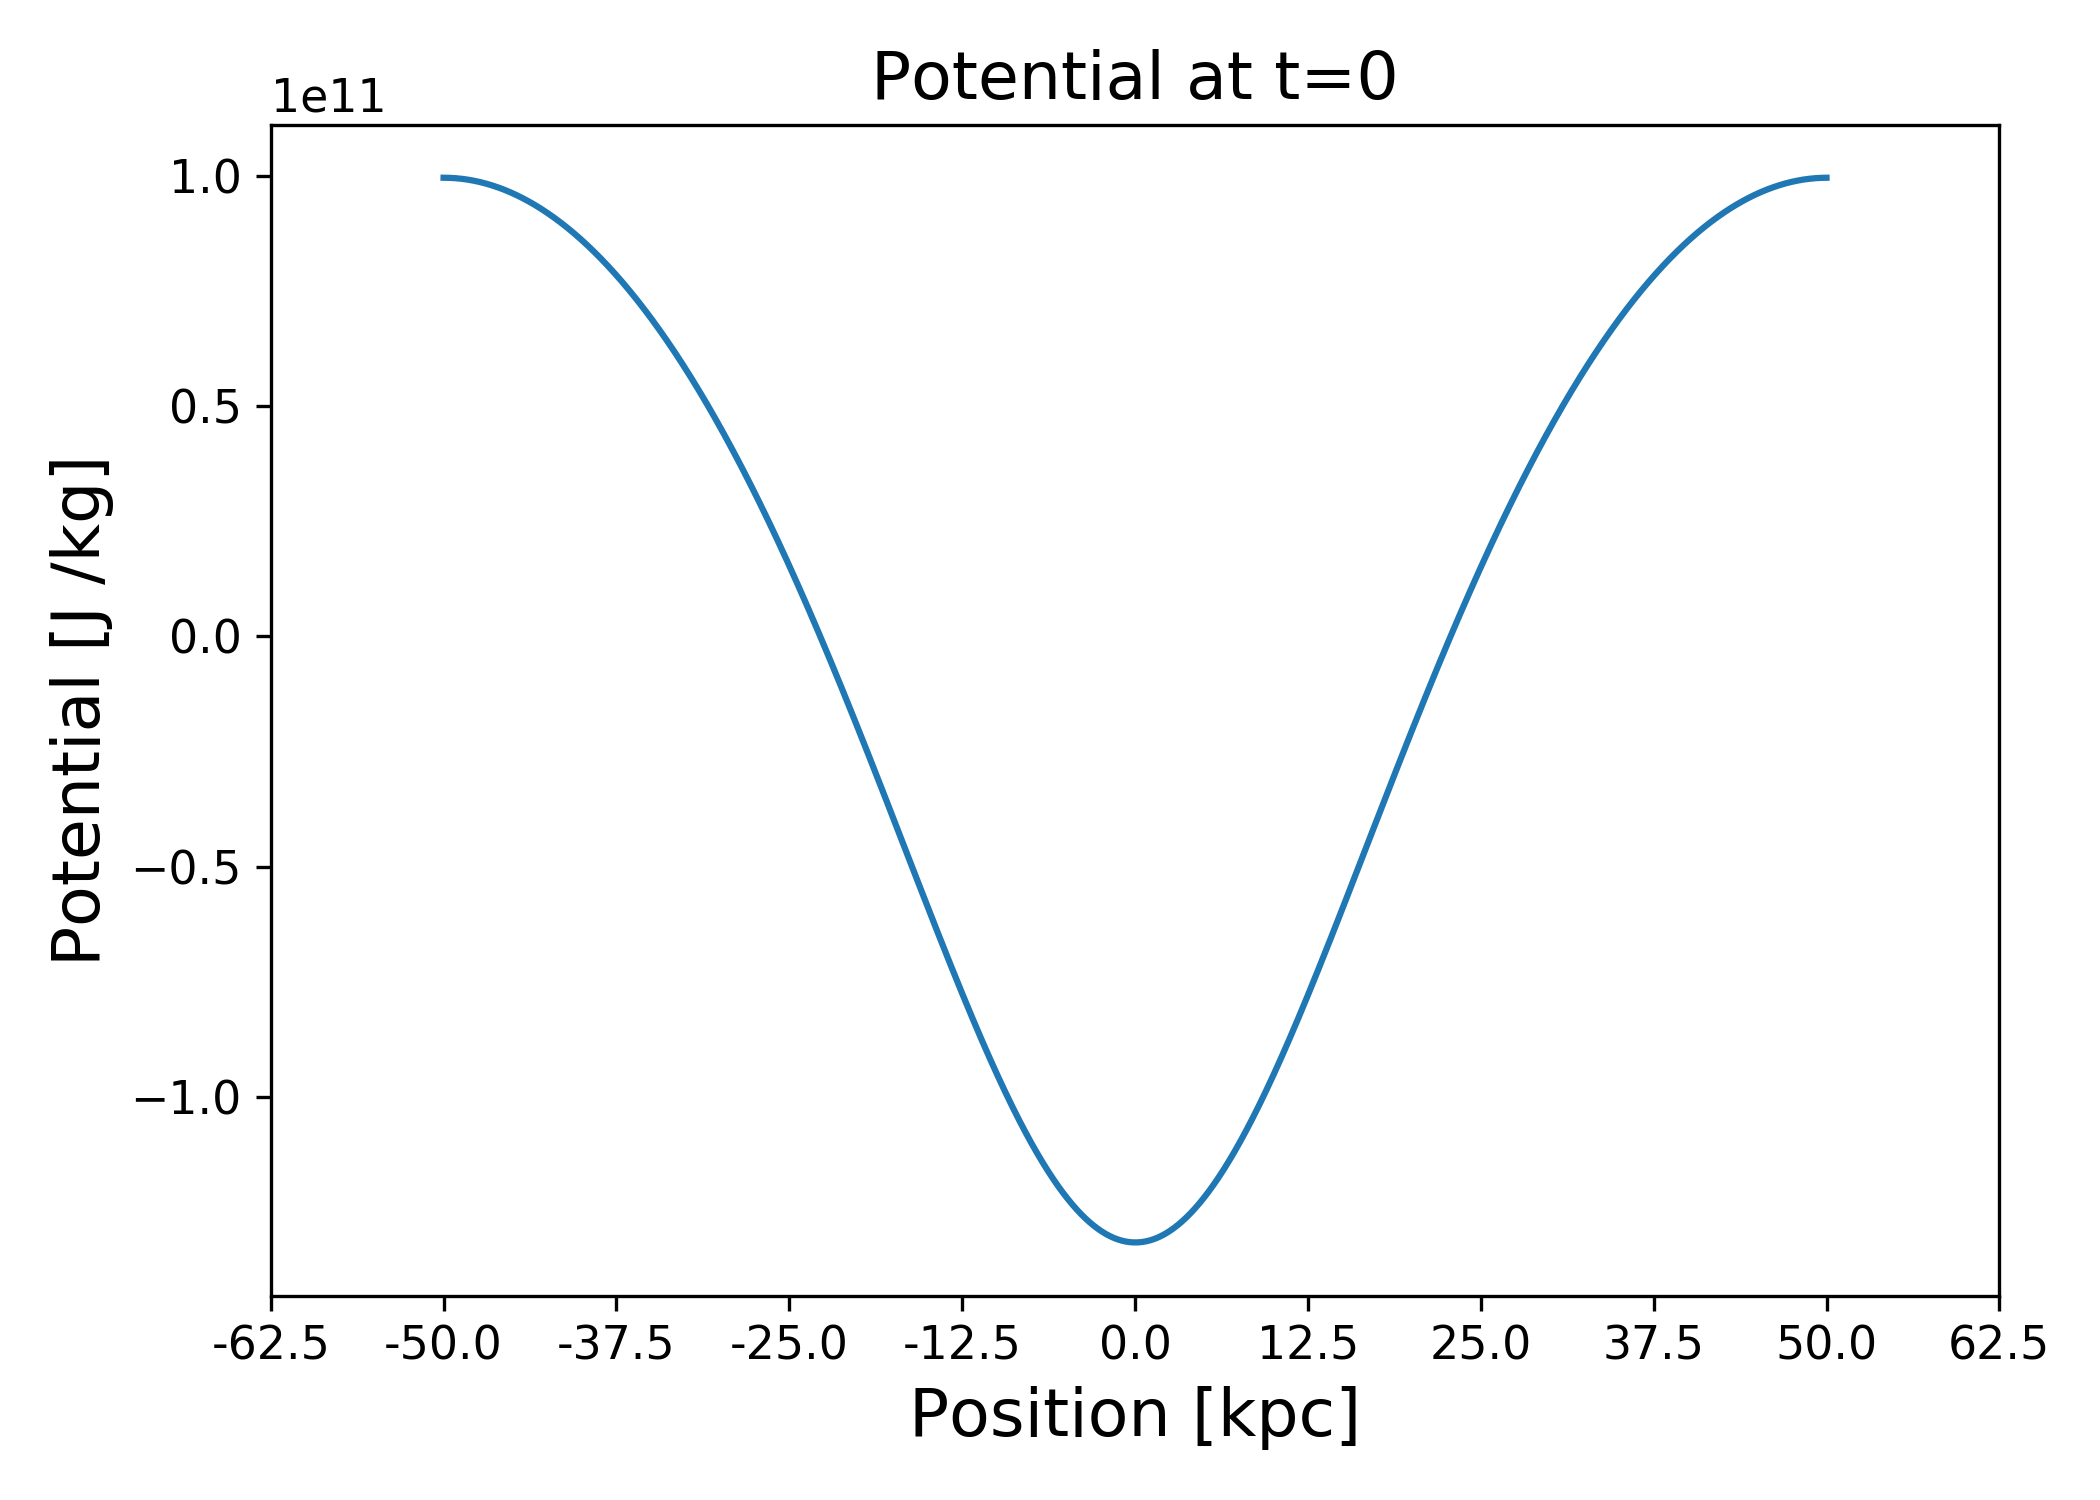
\includegraphics[scale=0.6]{imag/1dInitPot.png}
    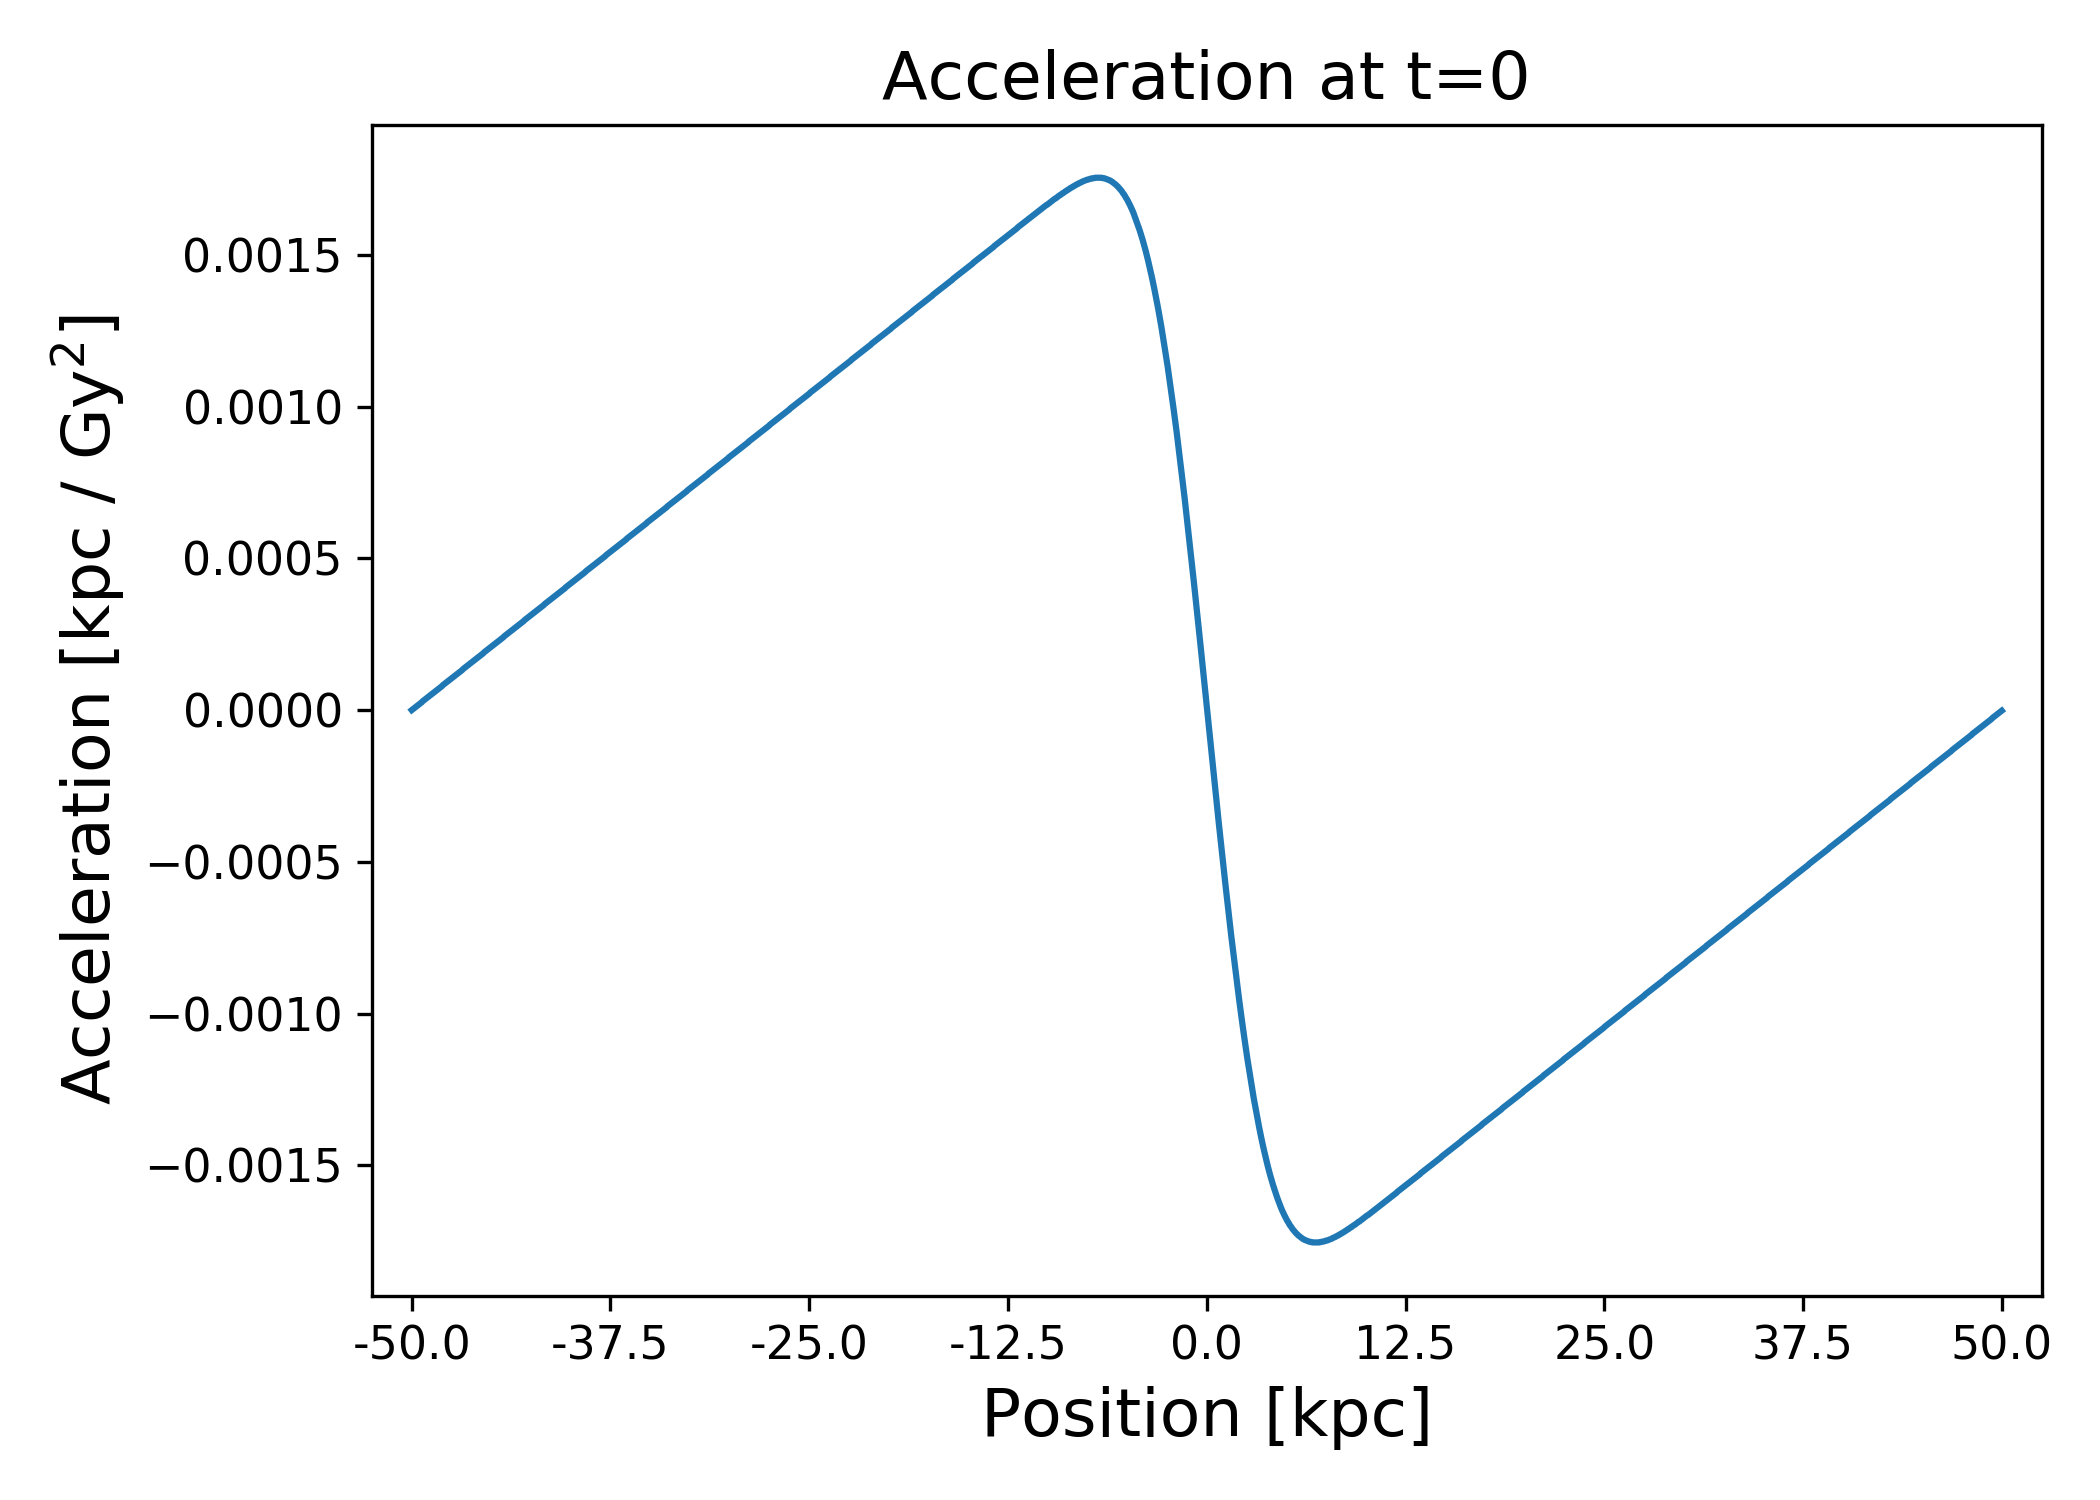
\includegraphics[scale=0.6]{imag/1dInitAcce.png}
    \caption{Up: The potential obtained by solving the Poisson equation. Given that the density was a Gaussian profile, it is no surprise that the potential is a negative Gaussian profile. Down: The acceleration obtain by numerical derivation of the potential.}
    \label{1dInit2}
\end{figure}

To test the simulation we reproduce previous work in the collisionless case. For which we run the simulation and check upon the behavior of the phase space density, the spatial density, the potential and the acceleration. 
In the phase space grid, we expect the cells with positive velocity to move to the right side of the plot, but, as they move to the right they are also being attracted towards the left because of the symmetry of the initial conditions. Therefore, the cells with positive velocity will move towards the inferior-right side of the plot, while cells with negative velocity will move towards the upper left side of the phase space. Overall, the phase space behaves like a clockwise-rotating spiral. This spiral structure can be seen in figure \ref{1dphase}

\begin{figure}[h!]
    \centering
    %\includegraphics[width=10cm,height =7cm]{Diapositiva1.jpg}
    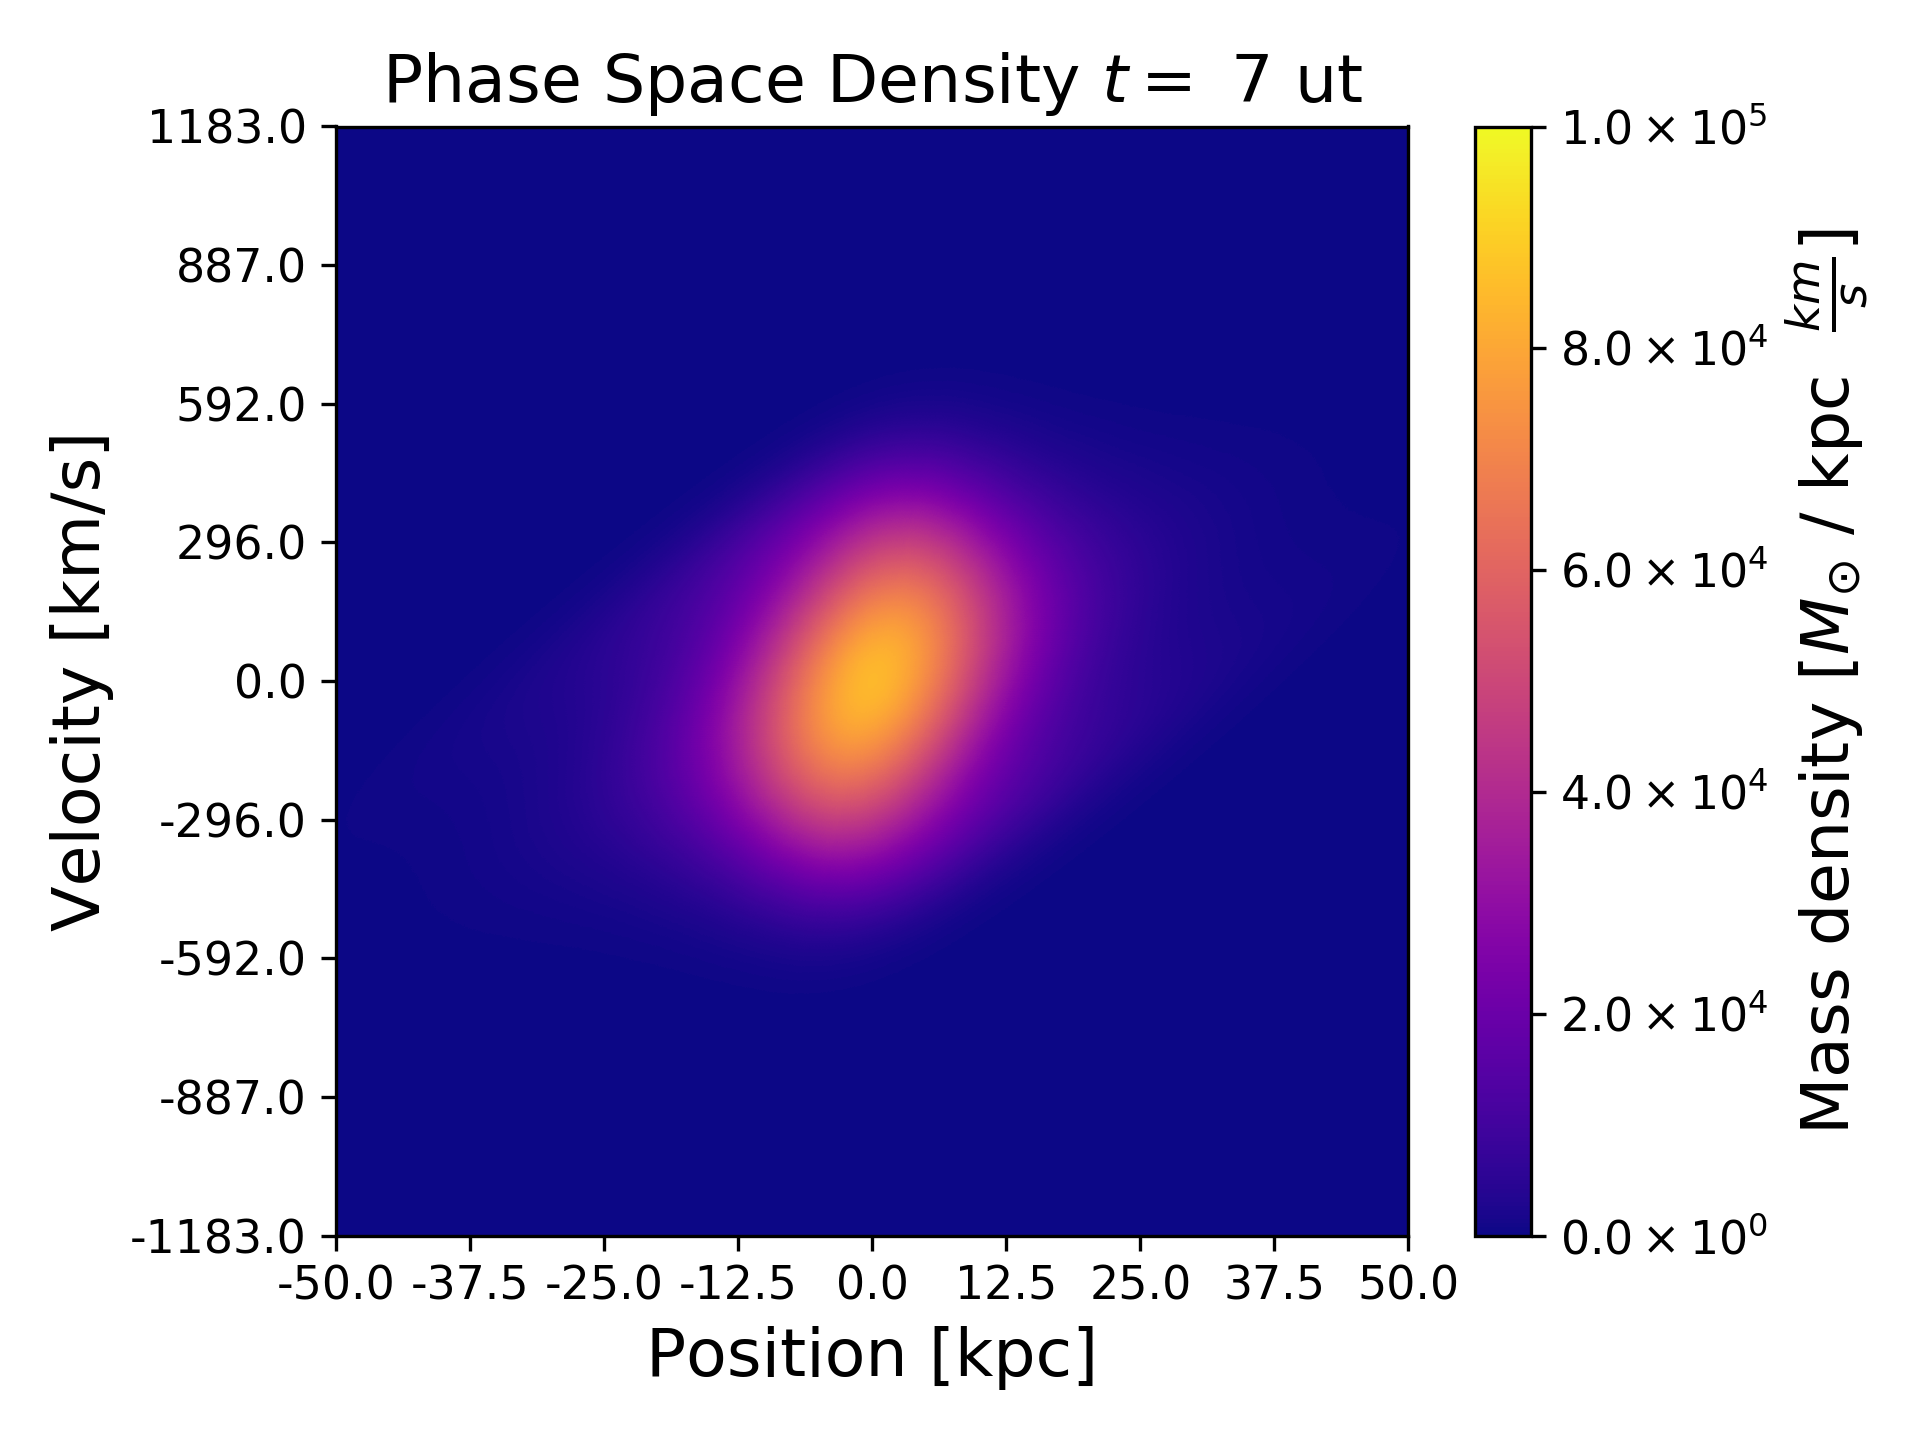
\includegraphics[scale=0.45]{imag/phase7.png}
    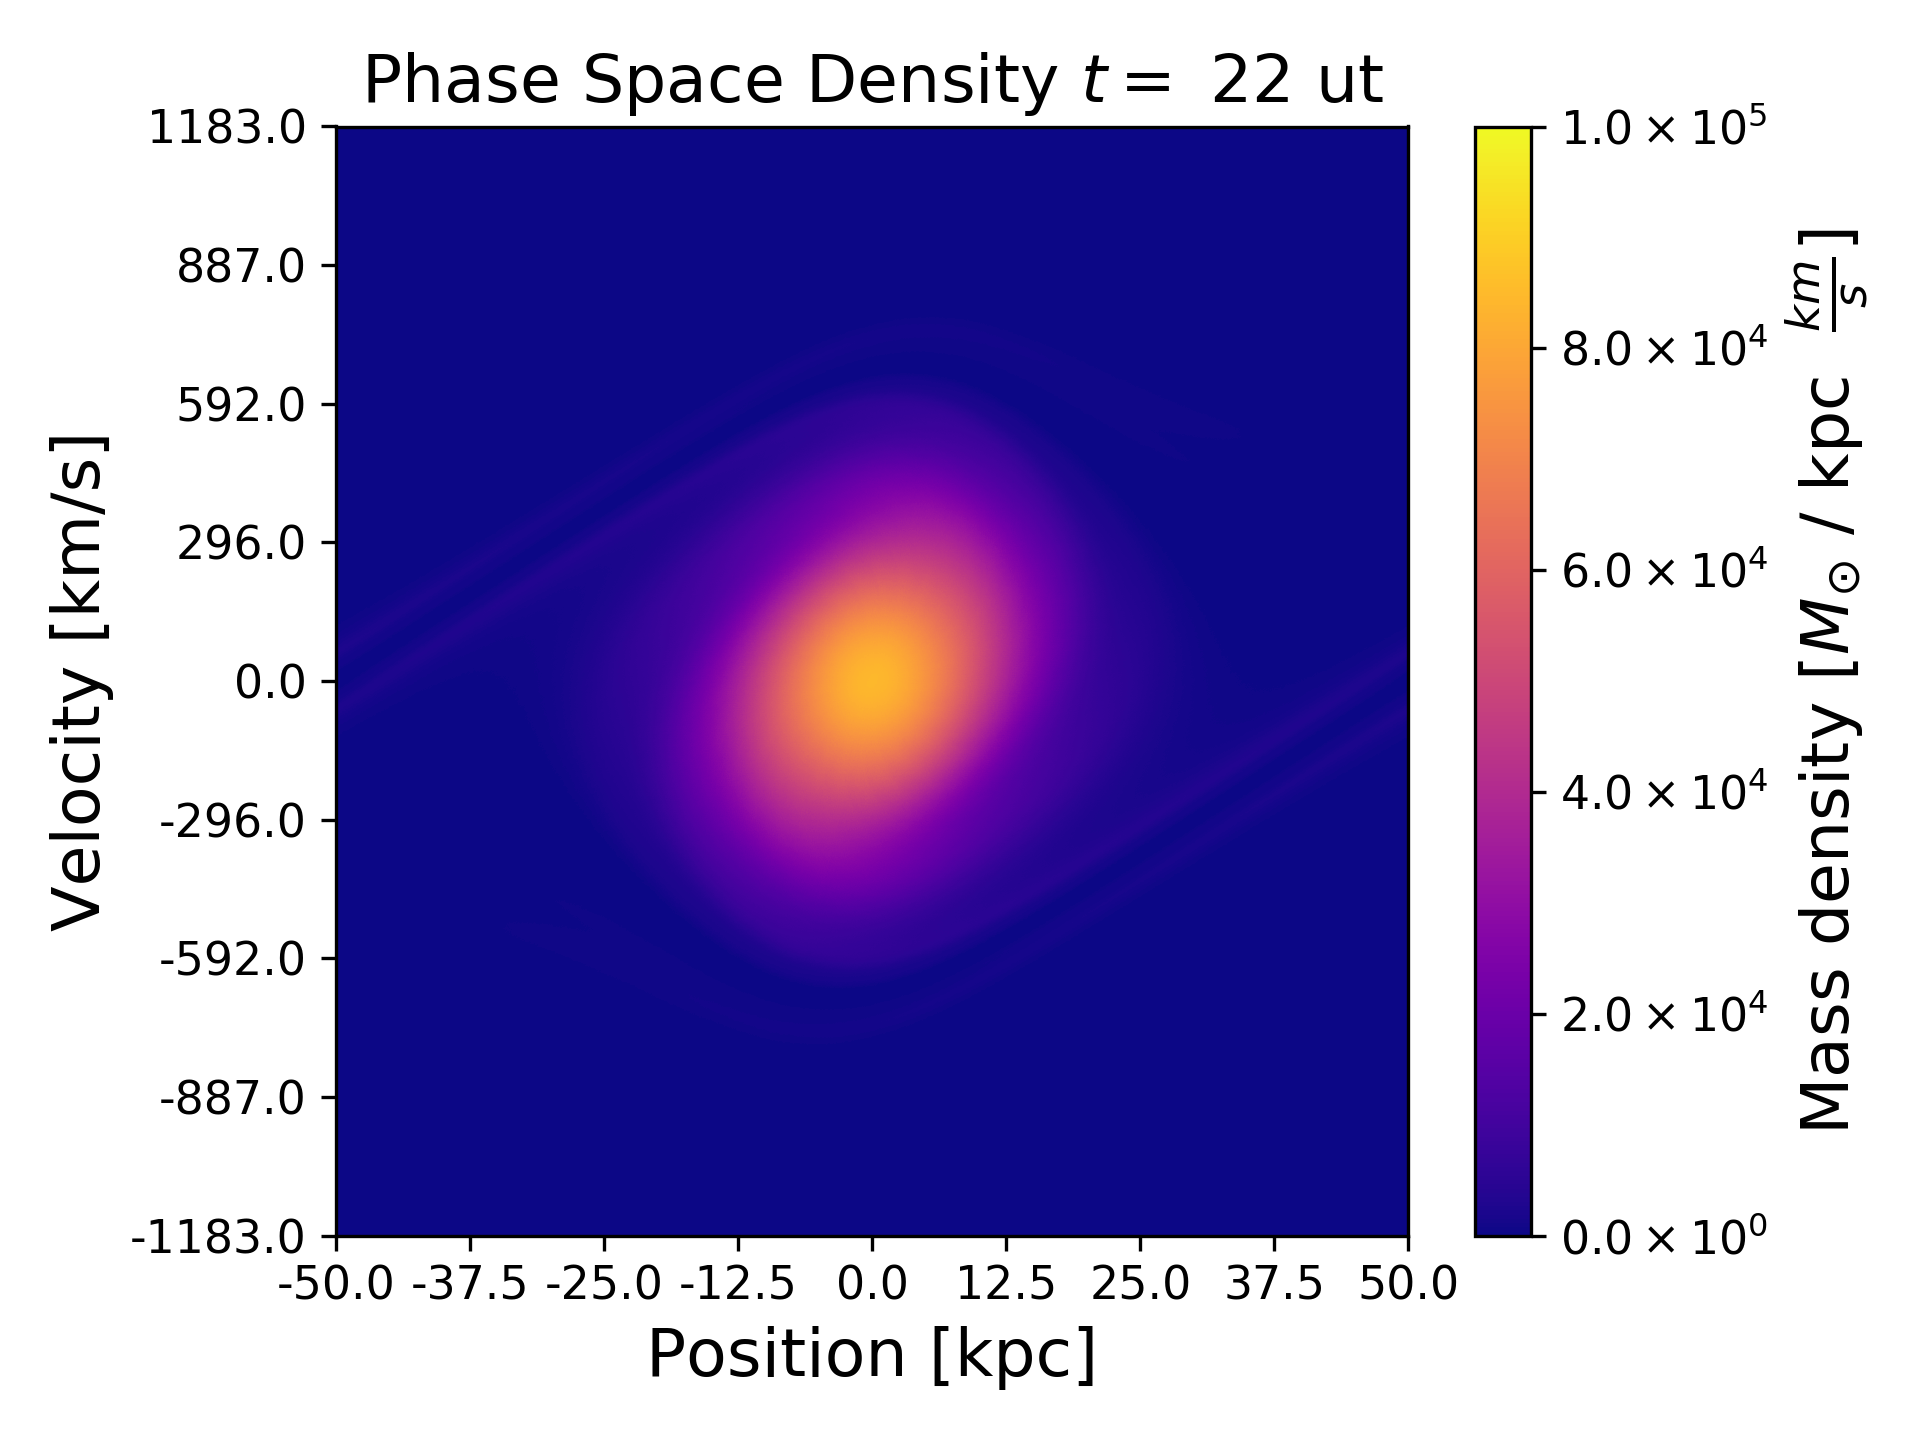
\includegraphics[scale=0.45]{imag/phase22.png}
    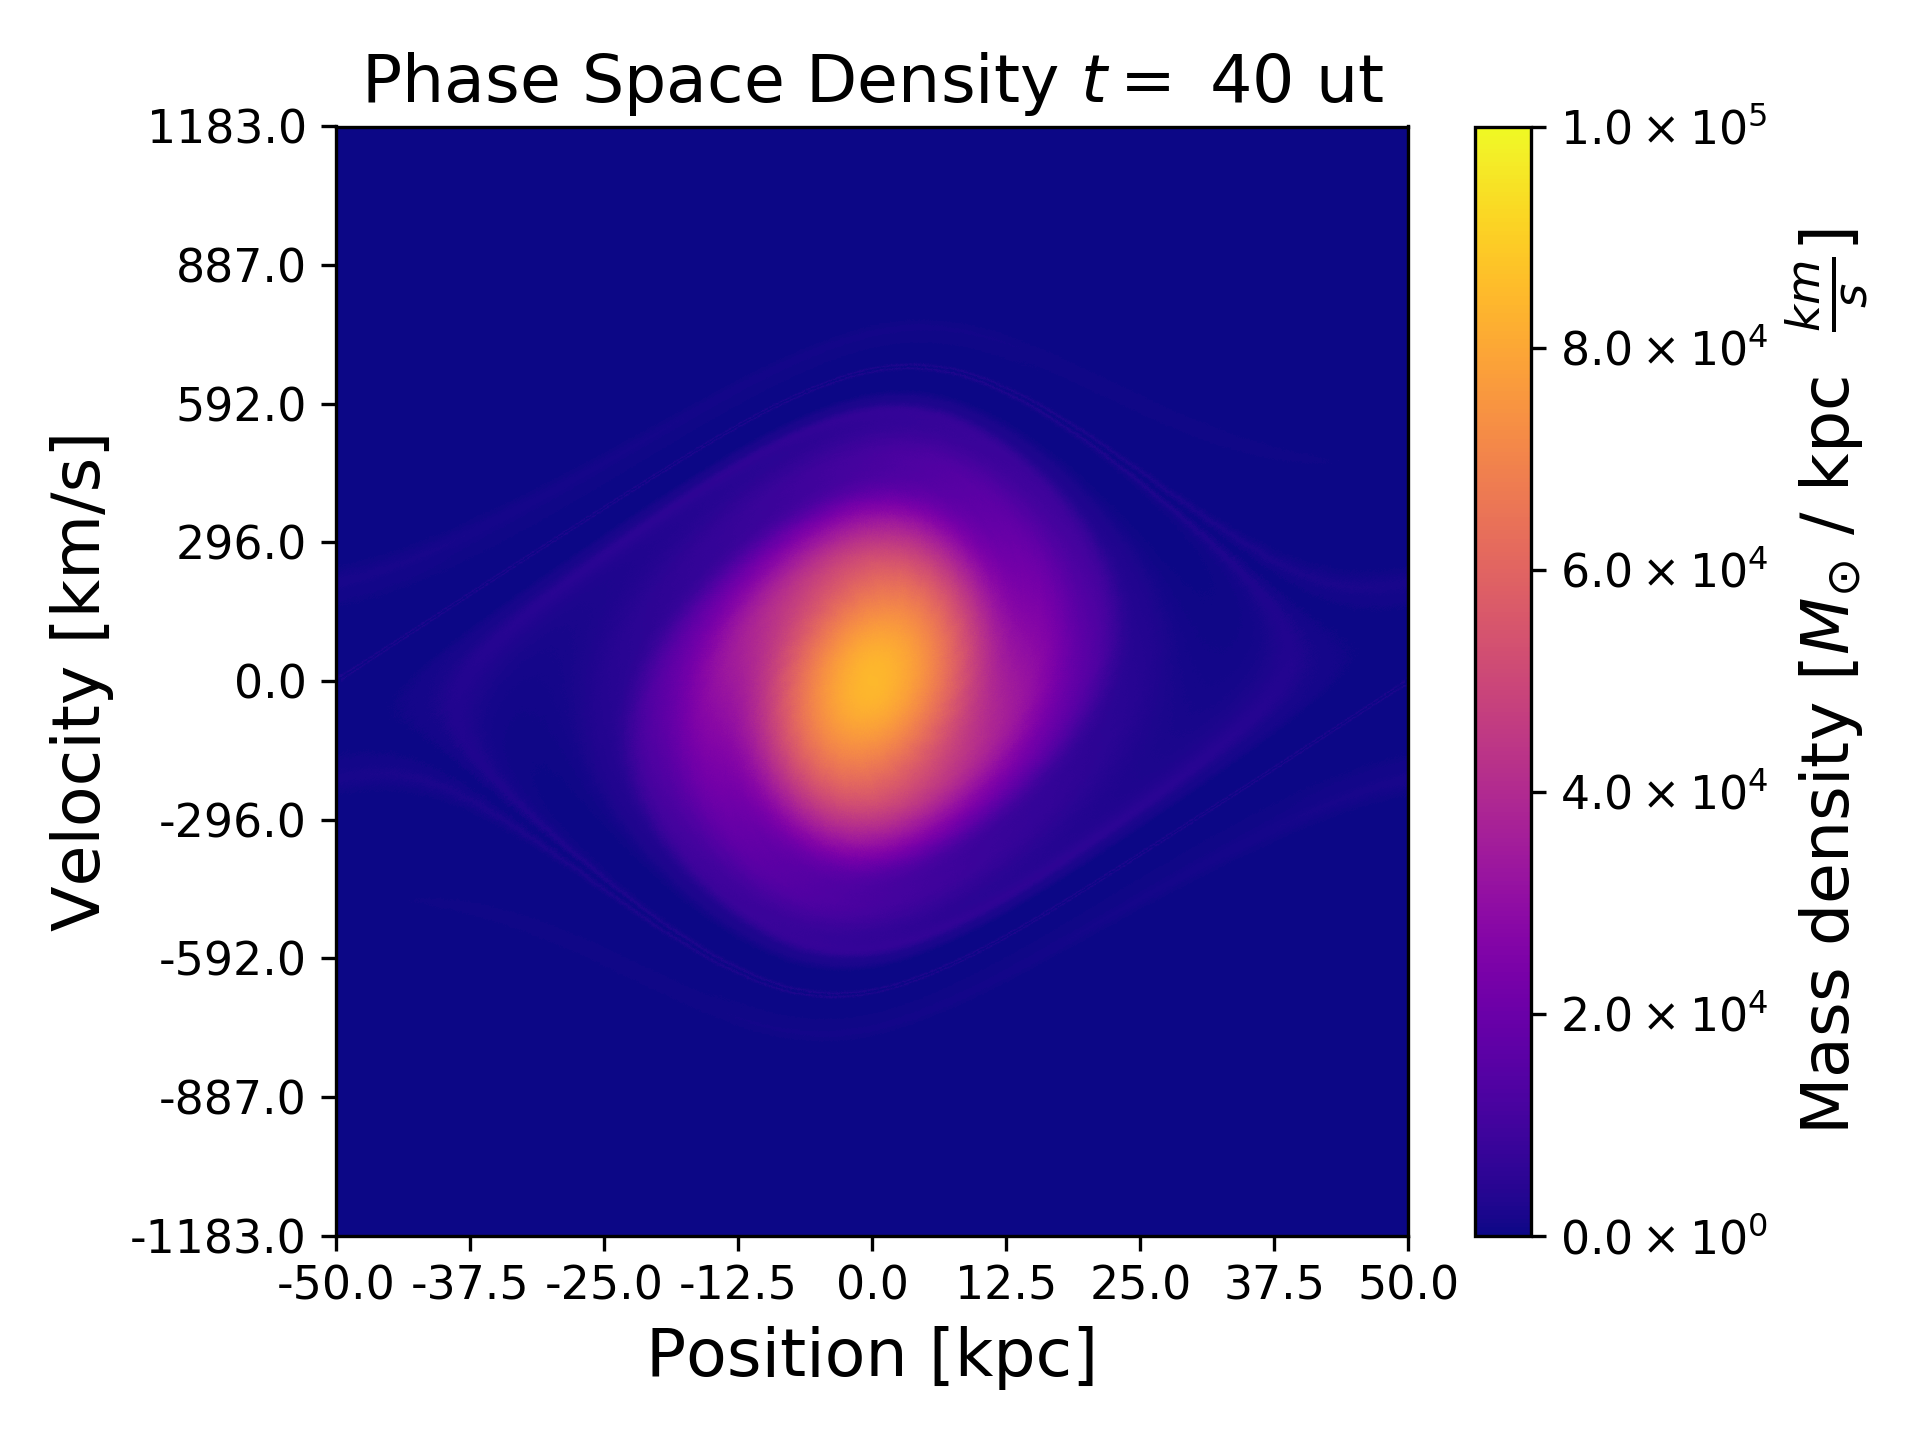
\includegraphics[scale=0.45]{imag/phase40.png}
    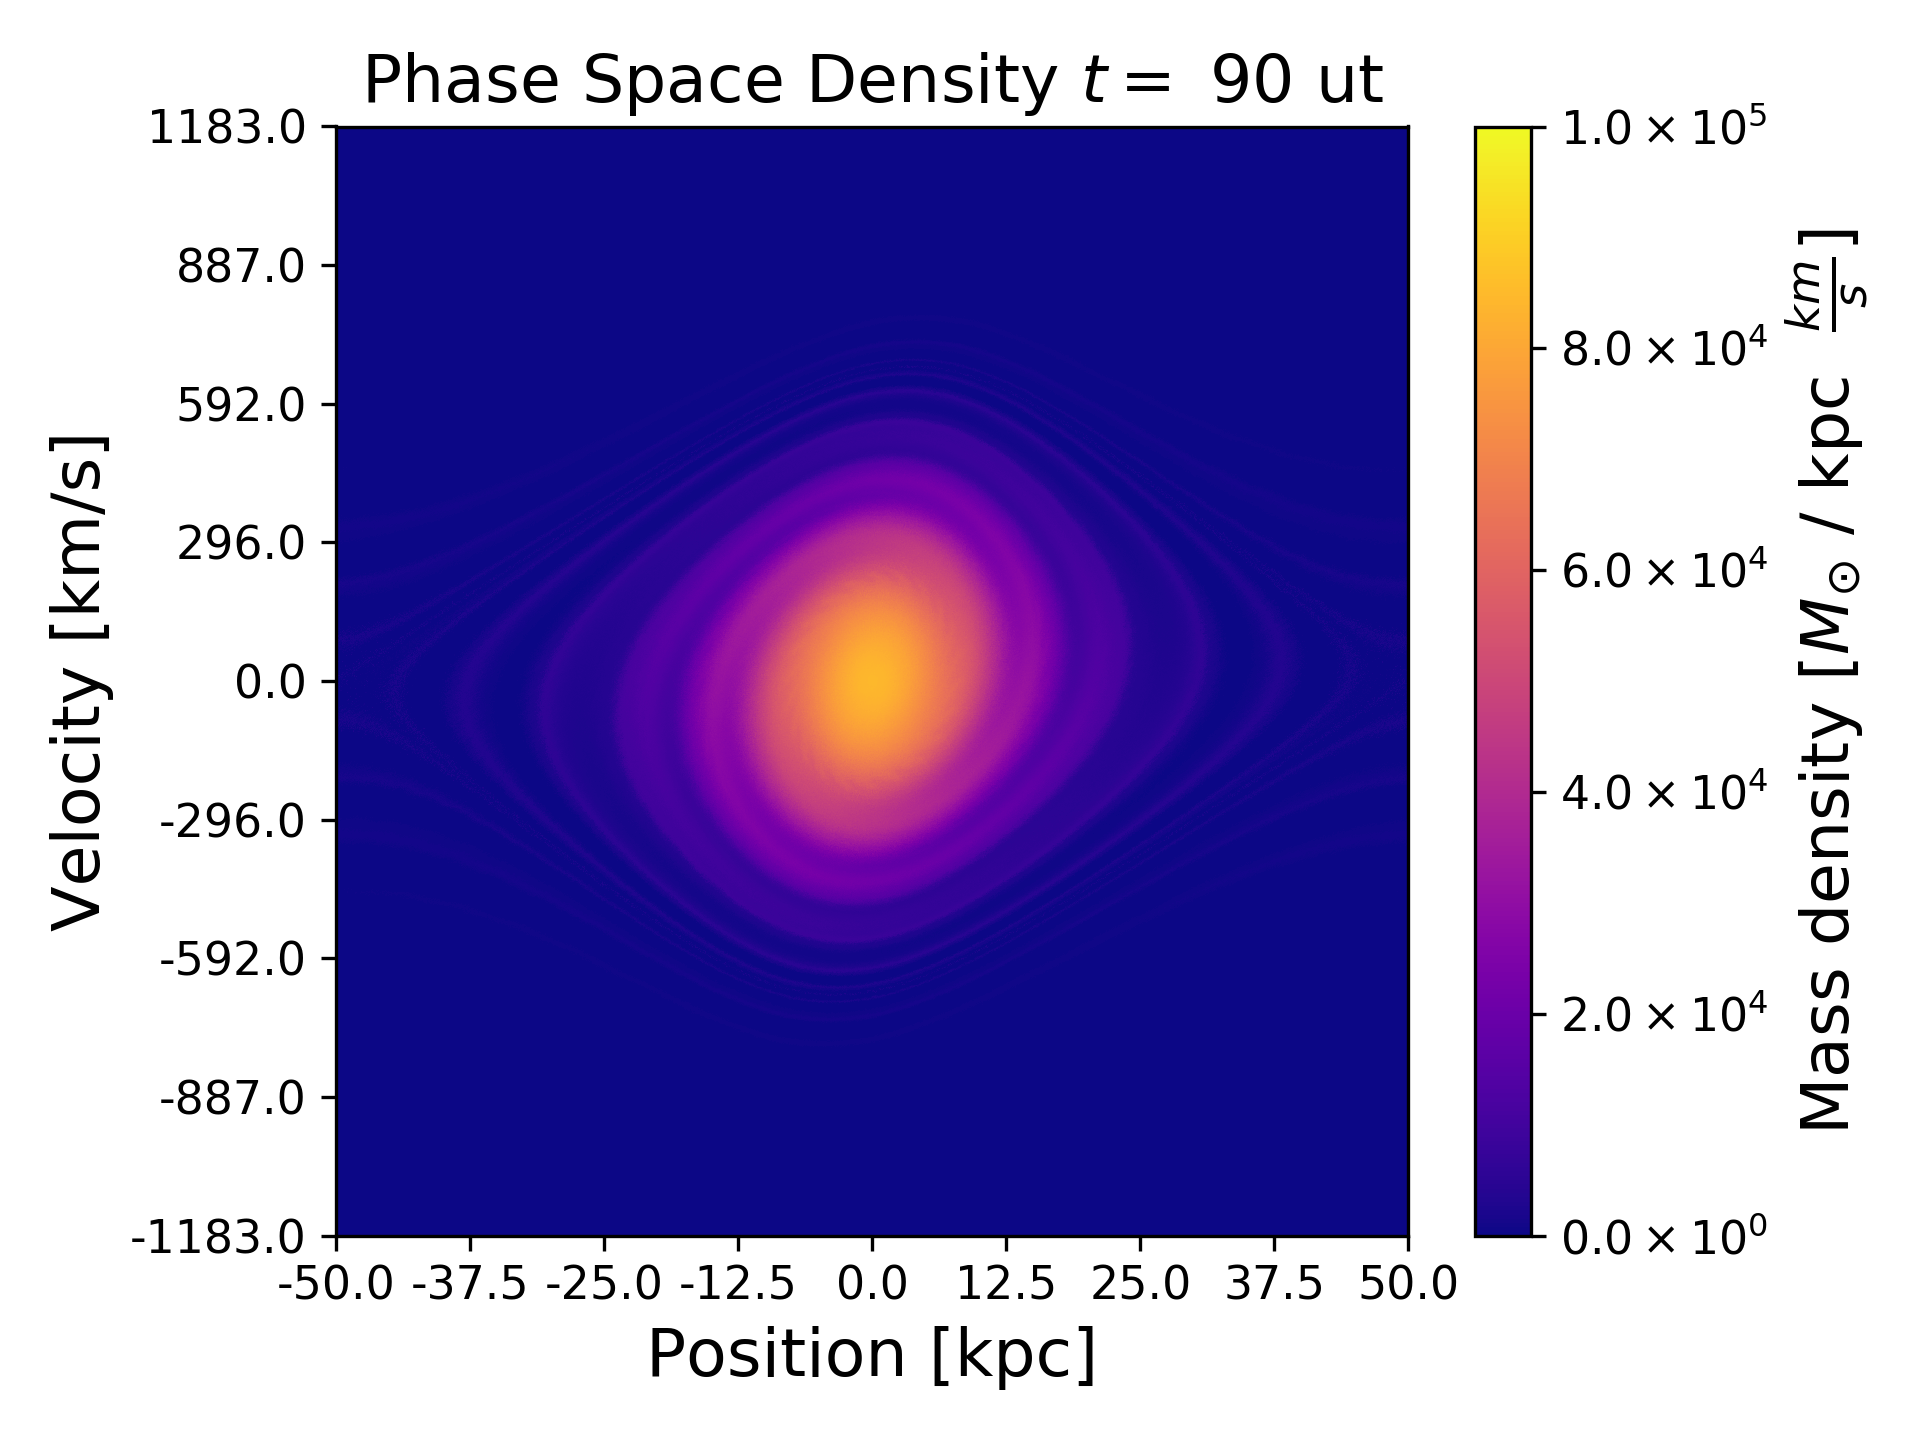
\includegraphics[scale=0.45]{imag/phase90.png}
    \caption{Upper left: Phase space 72 million years after initialization. Upper right: Phase space 227 million years after initialization. Bottom left: Phase space 413 million years after initialization. Bottom right: Phase space 930 million years after initialization. It can be observed that the phase space behaves as a clock-wise rotating spiral.}
    \label{1dphase}
\end{figure}


Overall, the trajectories in the phase space are a clock-wise rotating spiral. This behavior is in complete accordance with previous work and can be seen in figure \ref{1dphase}, where we plot different time instants chosen to display the clock-wise spiral of the phase space evolution.

To visualize the linear density, we plot the linear density vs position. We observe an initial increase in the height of the central peak and then little bumps trying to abandon the central distribution but they are gravitationally pulled back before crossing the spatial boundaries. This behavior can be seen in figure \ref{1dDens}




\begin{figure}[h!]
    \centering
    %\includegraphics[width=10cm,height =7cm]{Diapositiva1.jpg}
    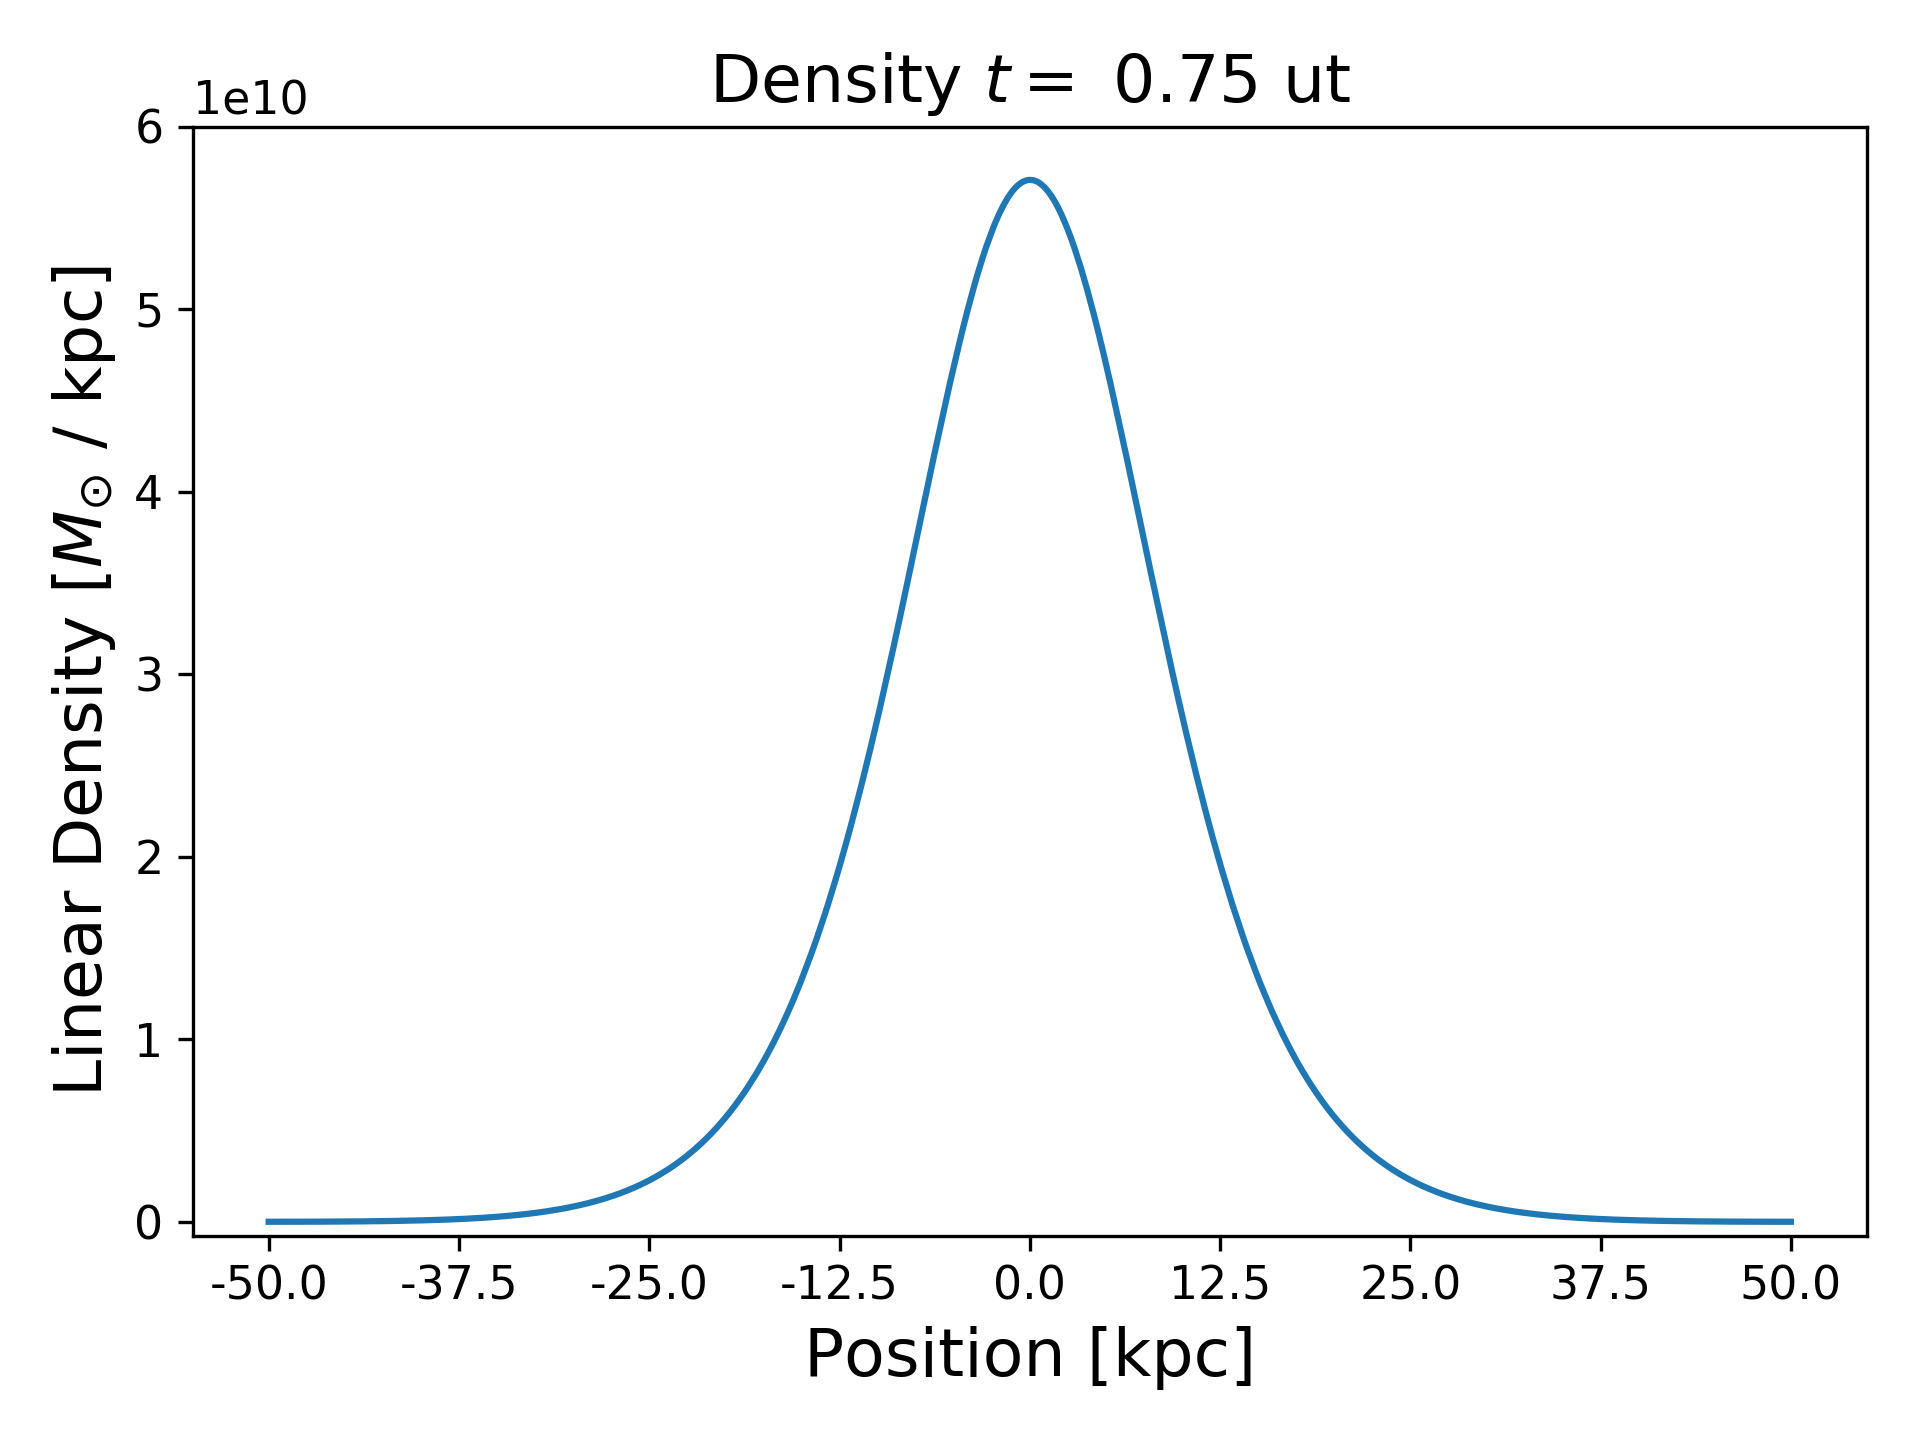
\includegraphics[scale=0.45]{imag/gaussD3.png}
    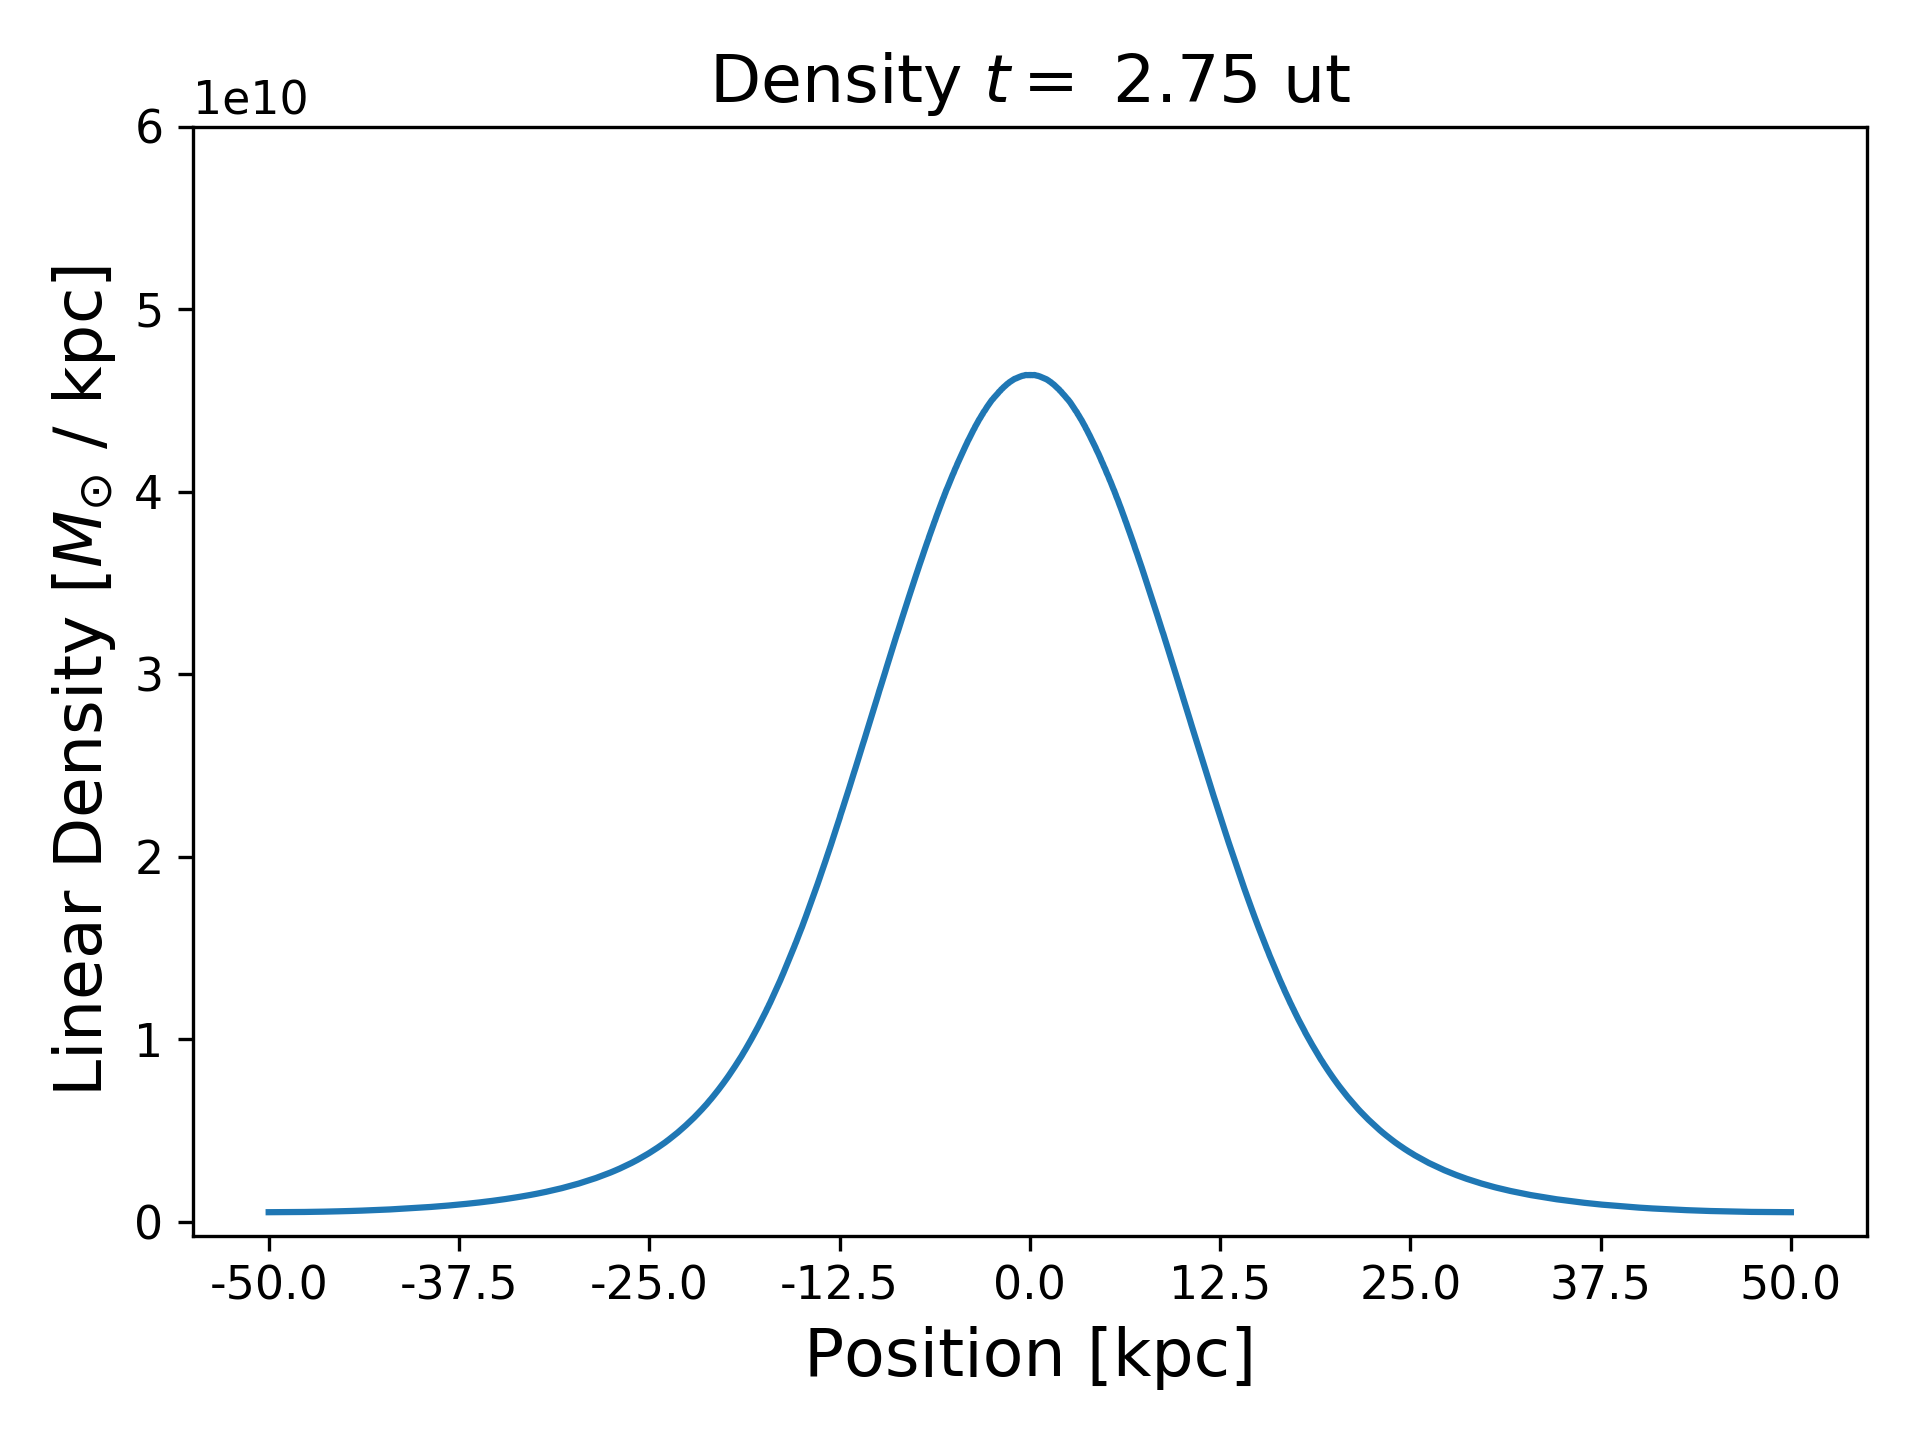
\includegraphics[scale=0.45]{imag/gaussD11.png}
    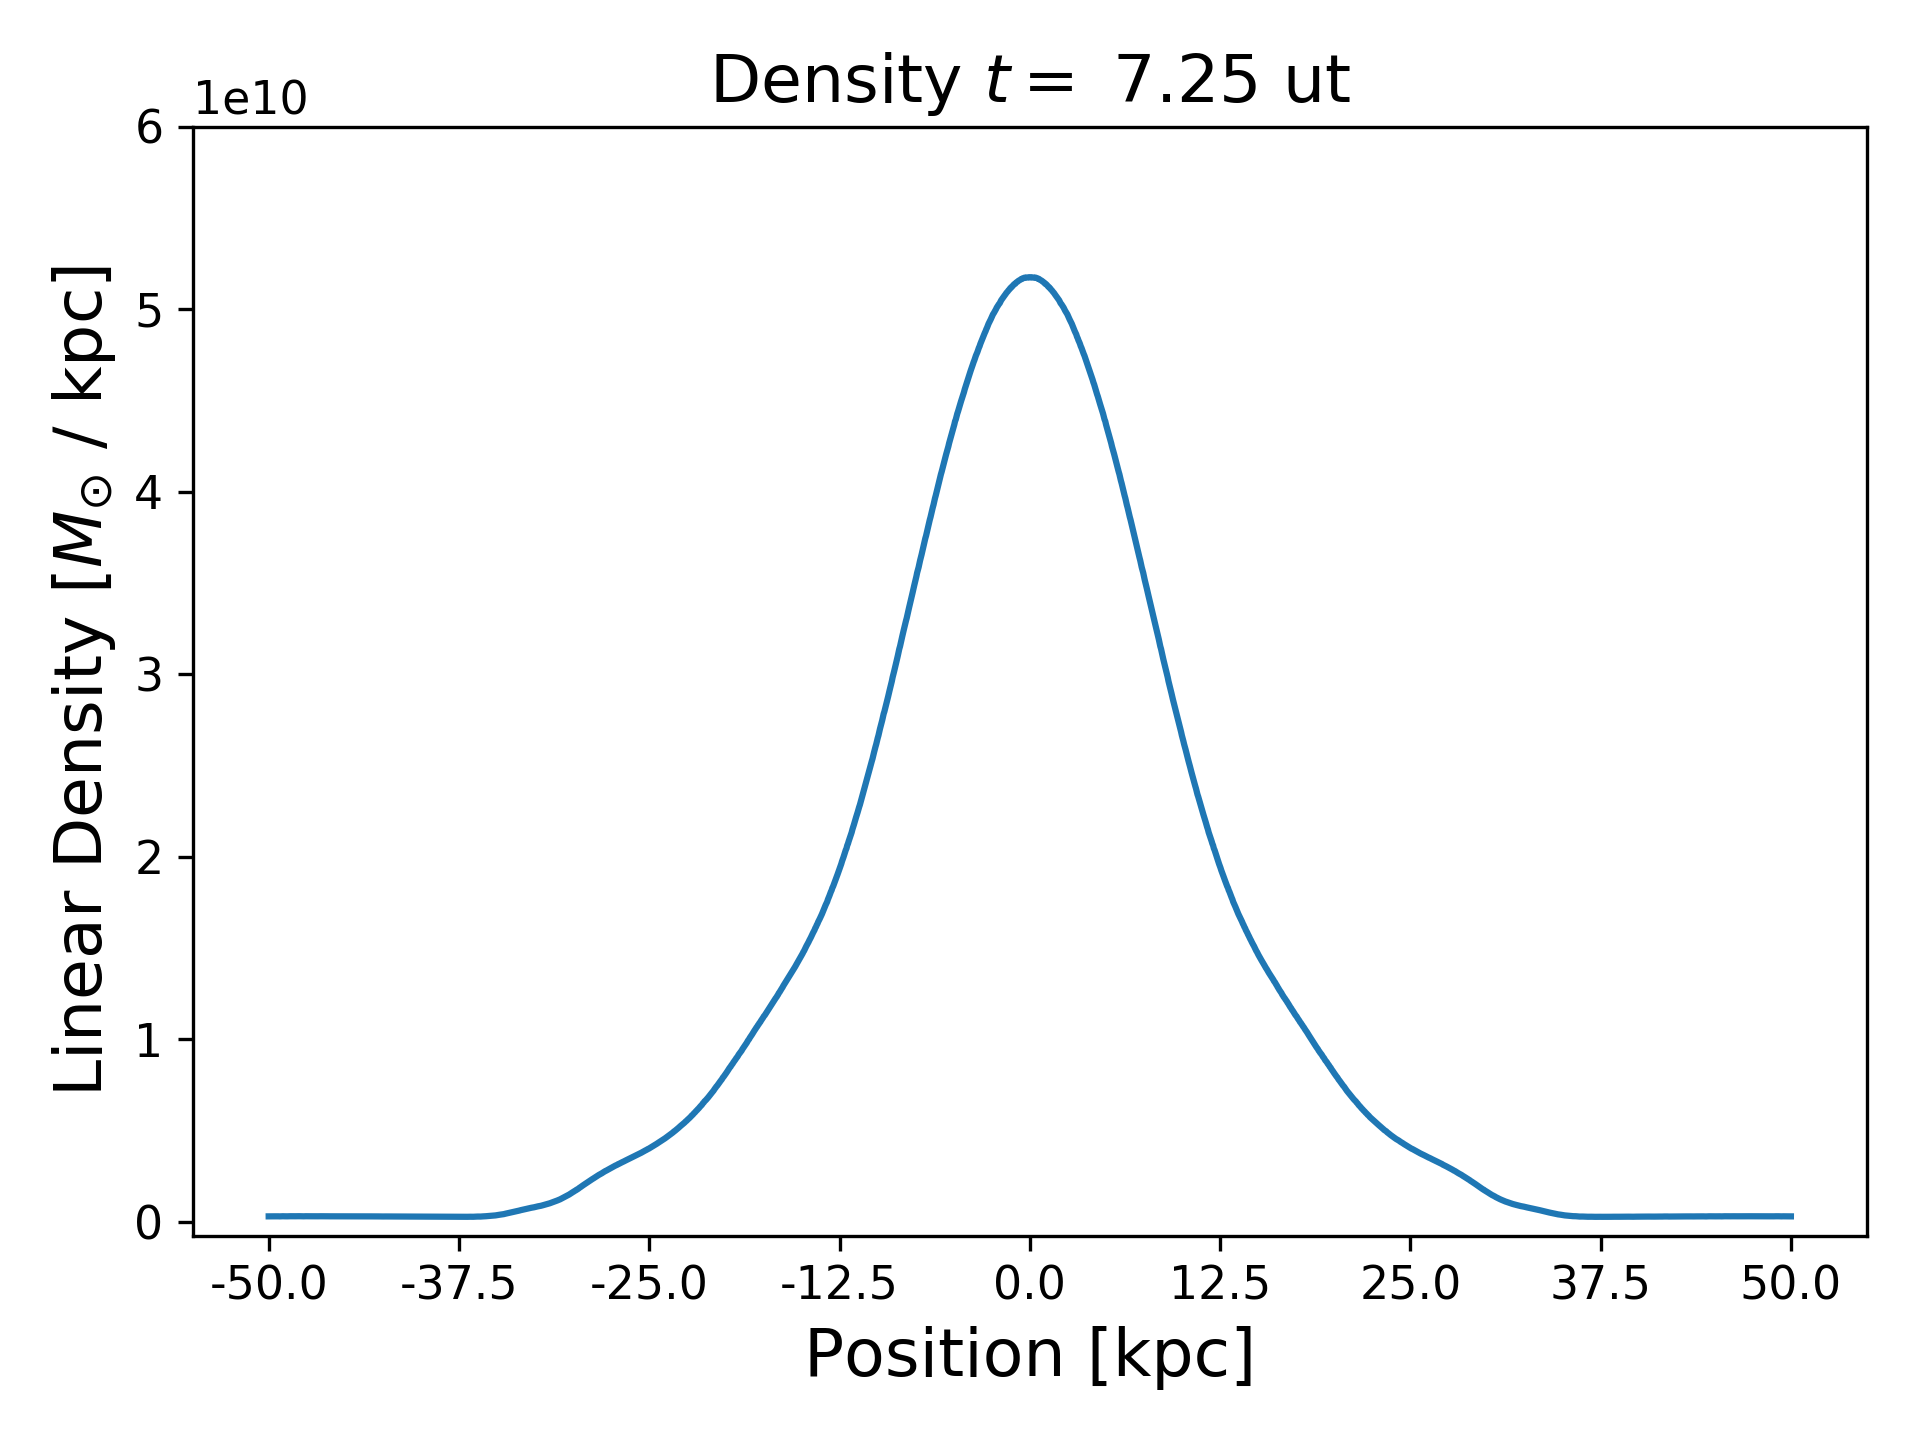
\includegraphics[scale=0.45]{imag/gaussD29.png}
    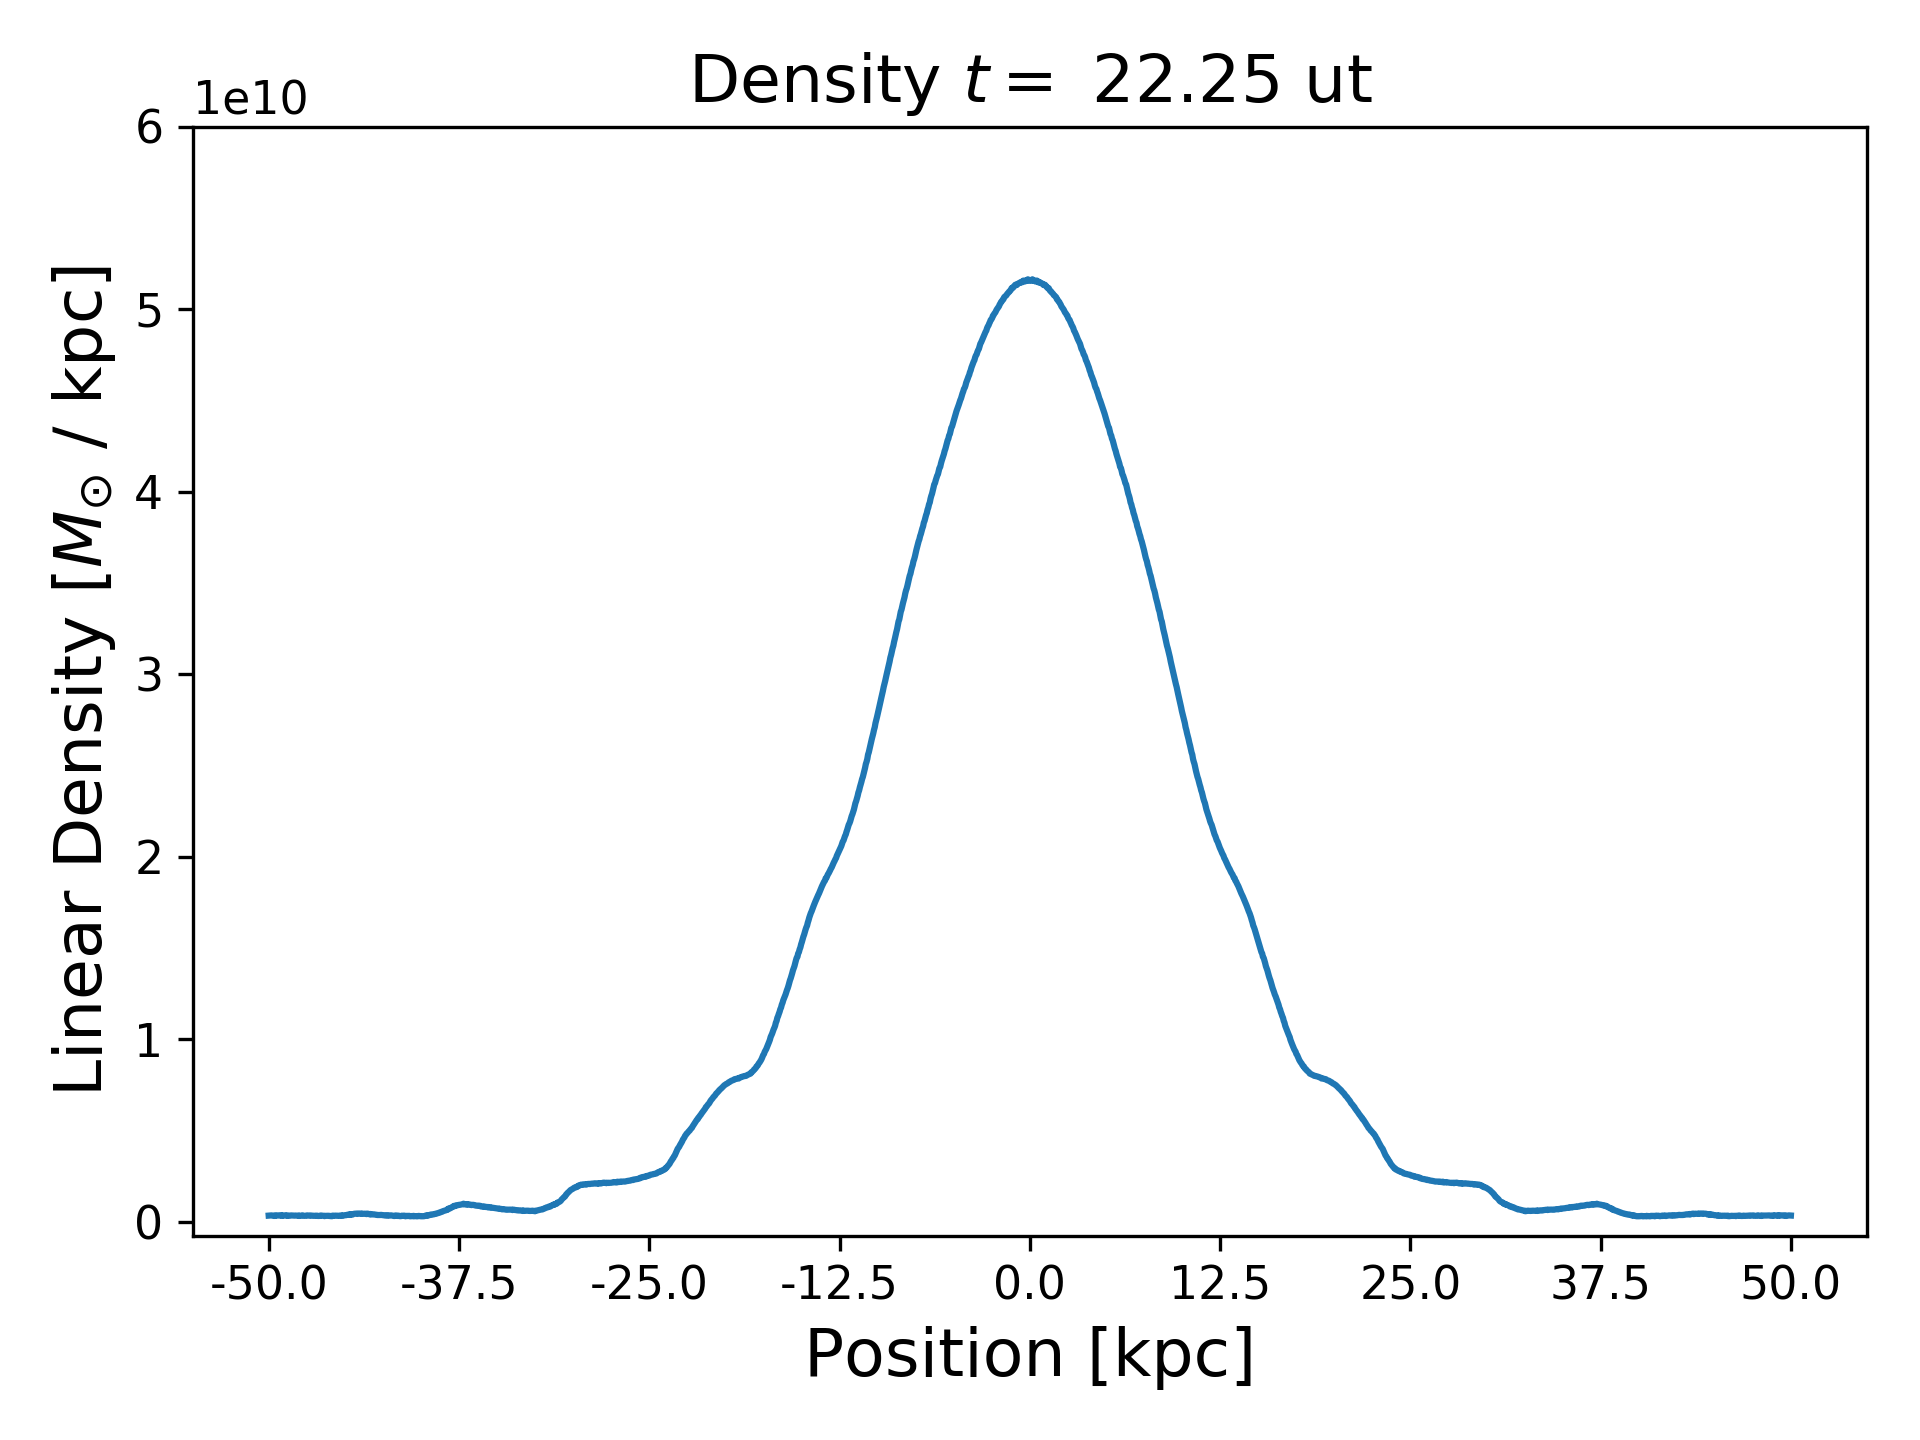
\includegraphics[scale=0.45]{imag/gaussD89.png}
    \caption{Upper left: linear density with its central peak at maximum height. Upper right: linear density the peak at a local minima after having reached maximum height . Bottom left: little bumps can be seen at the tails of the distribution. Bottom right: the tails of the distribution are completely bumpy and so is the base of the peak. The images are from 31, 114, 300 and 920 million years after initialization.  }
    \label{1dDens}
\end{figure}

In addition to testing Gaussian initial conditions, we reproduced the Jeans instability, which was also tested in previous work. In this scenario, the Jeans instability is given by:
\begin{equation}
f(r,v,0) = \frac{\bar{\rho}}{(2 \pi \sigma^2)^{1/2})} \exp(-\frac{v^2}{2 \sigma^2}) (1 + A \cos(kr))
\end{equation}\\
Such that $\rho$ is the average phase density of the system, $\sigma$ is a measure of the width of the velocity Gaussian profile, $A$ is the amplitude of the density fluctuation and $k$ is the wavenumber of the density fluctuation. We used the following values:
\begin{align}
\bar{\rho} &= 10 \  \text{um} \ \text{us}^{-1} \ (\text{us/ut})^{-1} \\
\sigma &= 0.1 \ \text{us} \\
A &= 0.9999 \\
k &= 2 \pi \ \text{us}^{-1}
\end{align}

For which the phase space behaved like three successive Gaussian profiles, that is because we meet the Jeans instability criteria. This result were also compatible with previous work published on one dimensional collisionless dark matter fluids. The evolution of the Jeans instability phase space can be seen in figure \ref{1dJeans}


\begin{figure}[h!]
    \centering
    %\includegraphics[width=10cm,height =7cm]{Diapositiva1.jpg}
    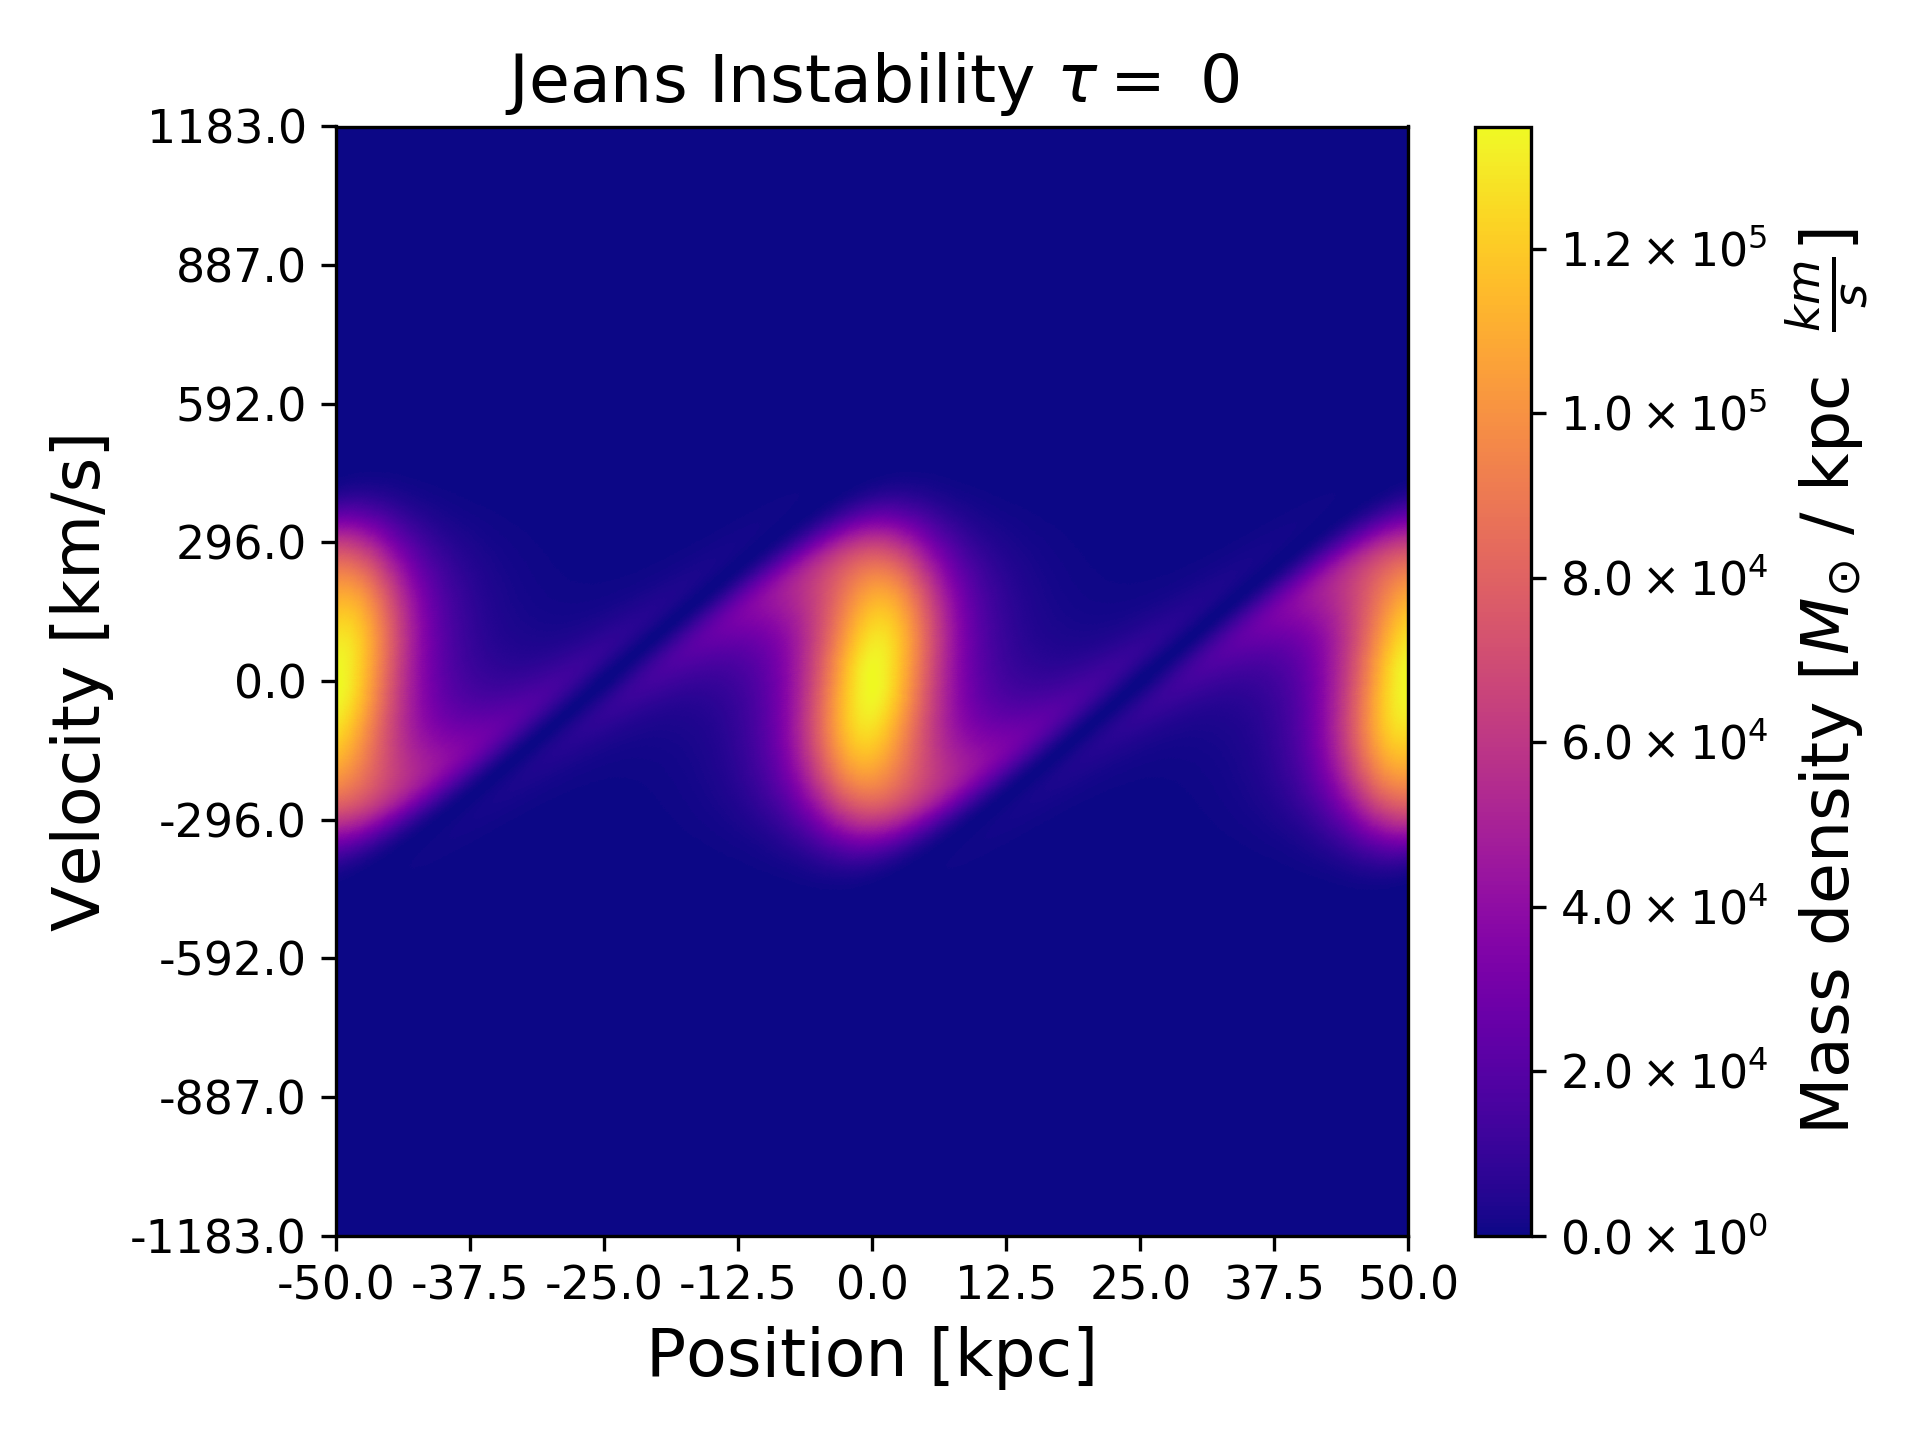
\includegraphics[scale=0.45]{imag/jeans7.png}
    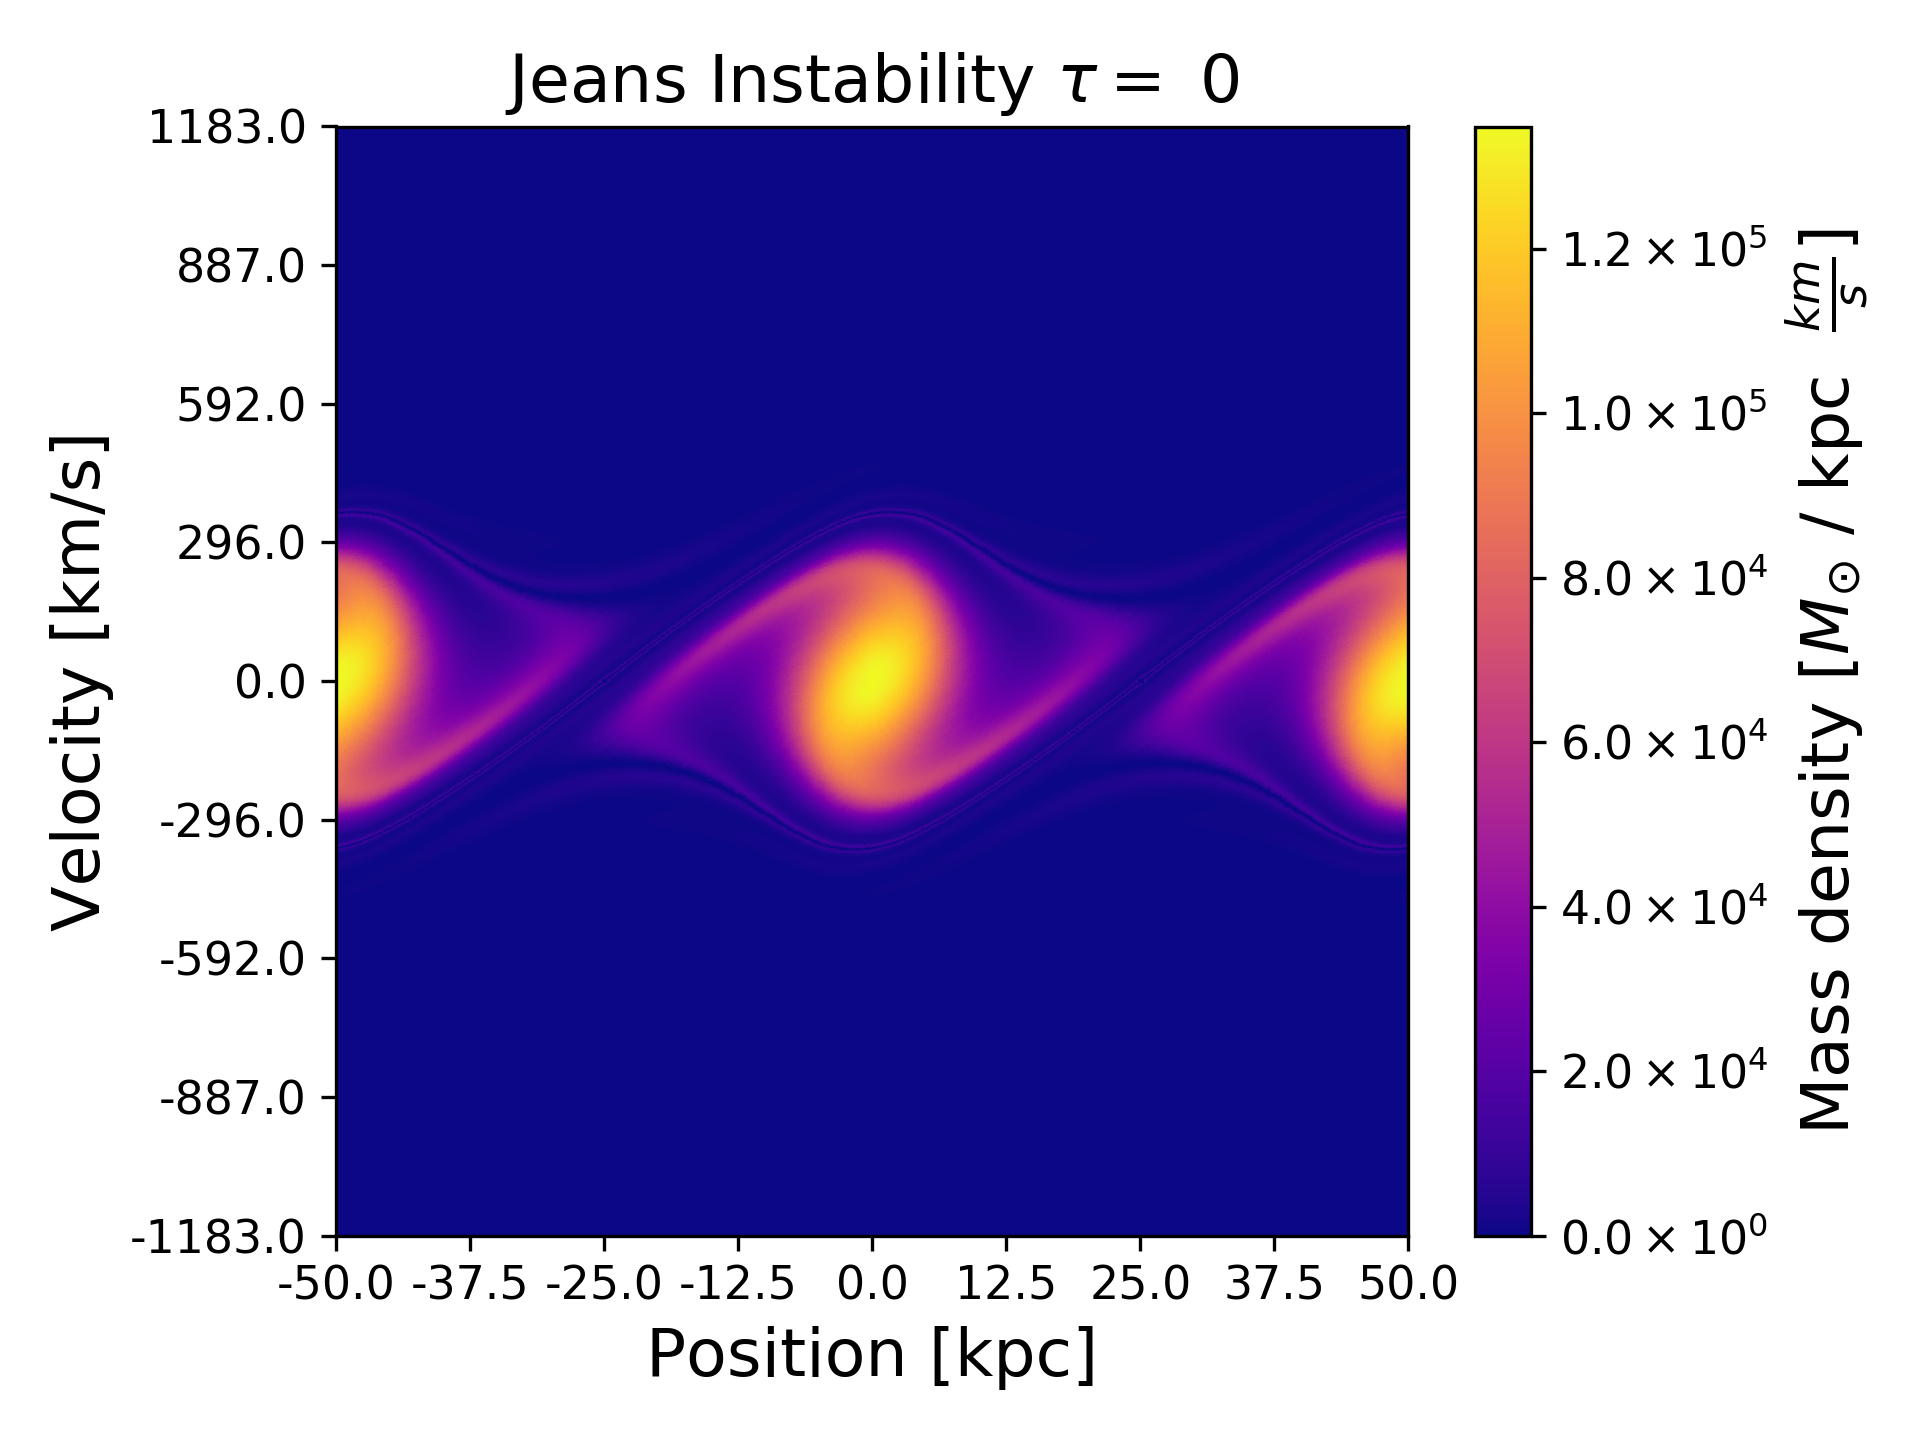
\includegraphics[scale=0.45]{imag/jeans22.png}
    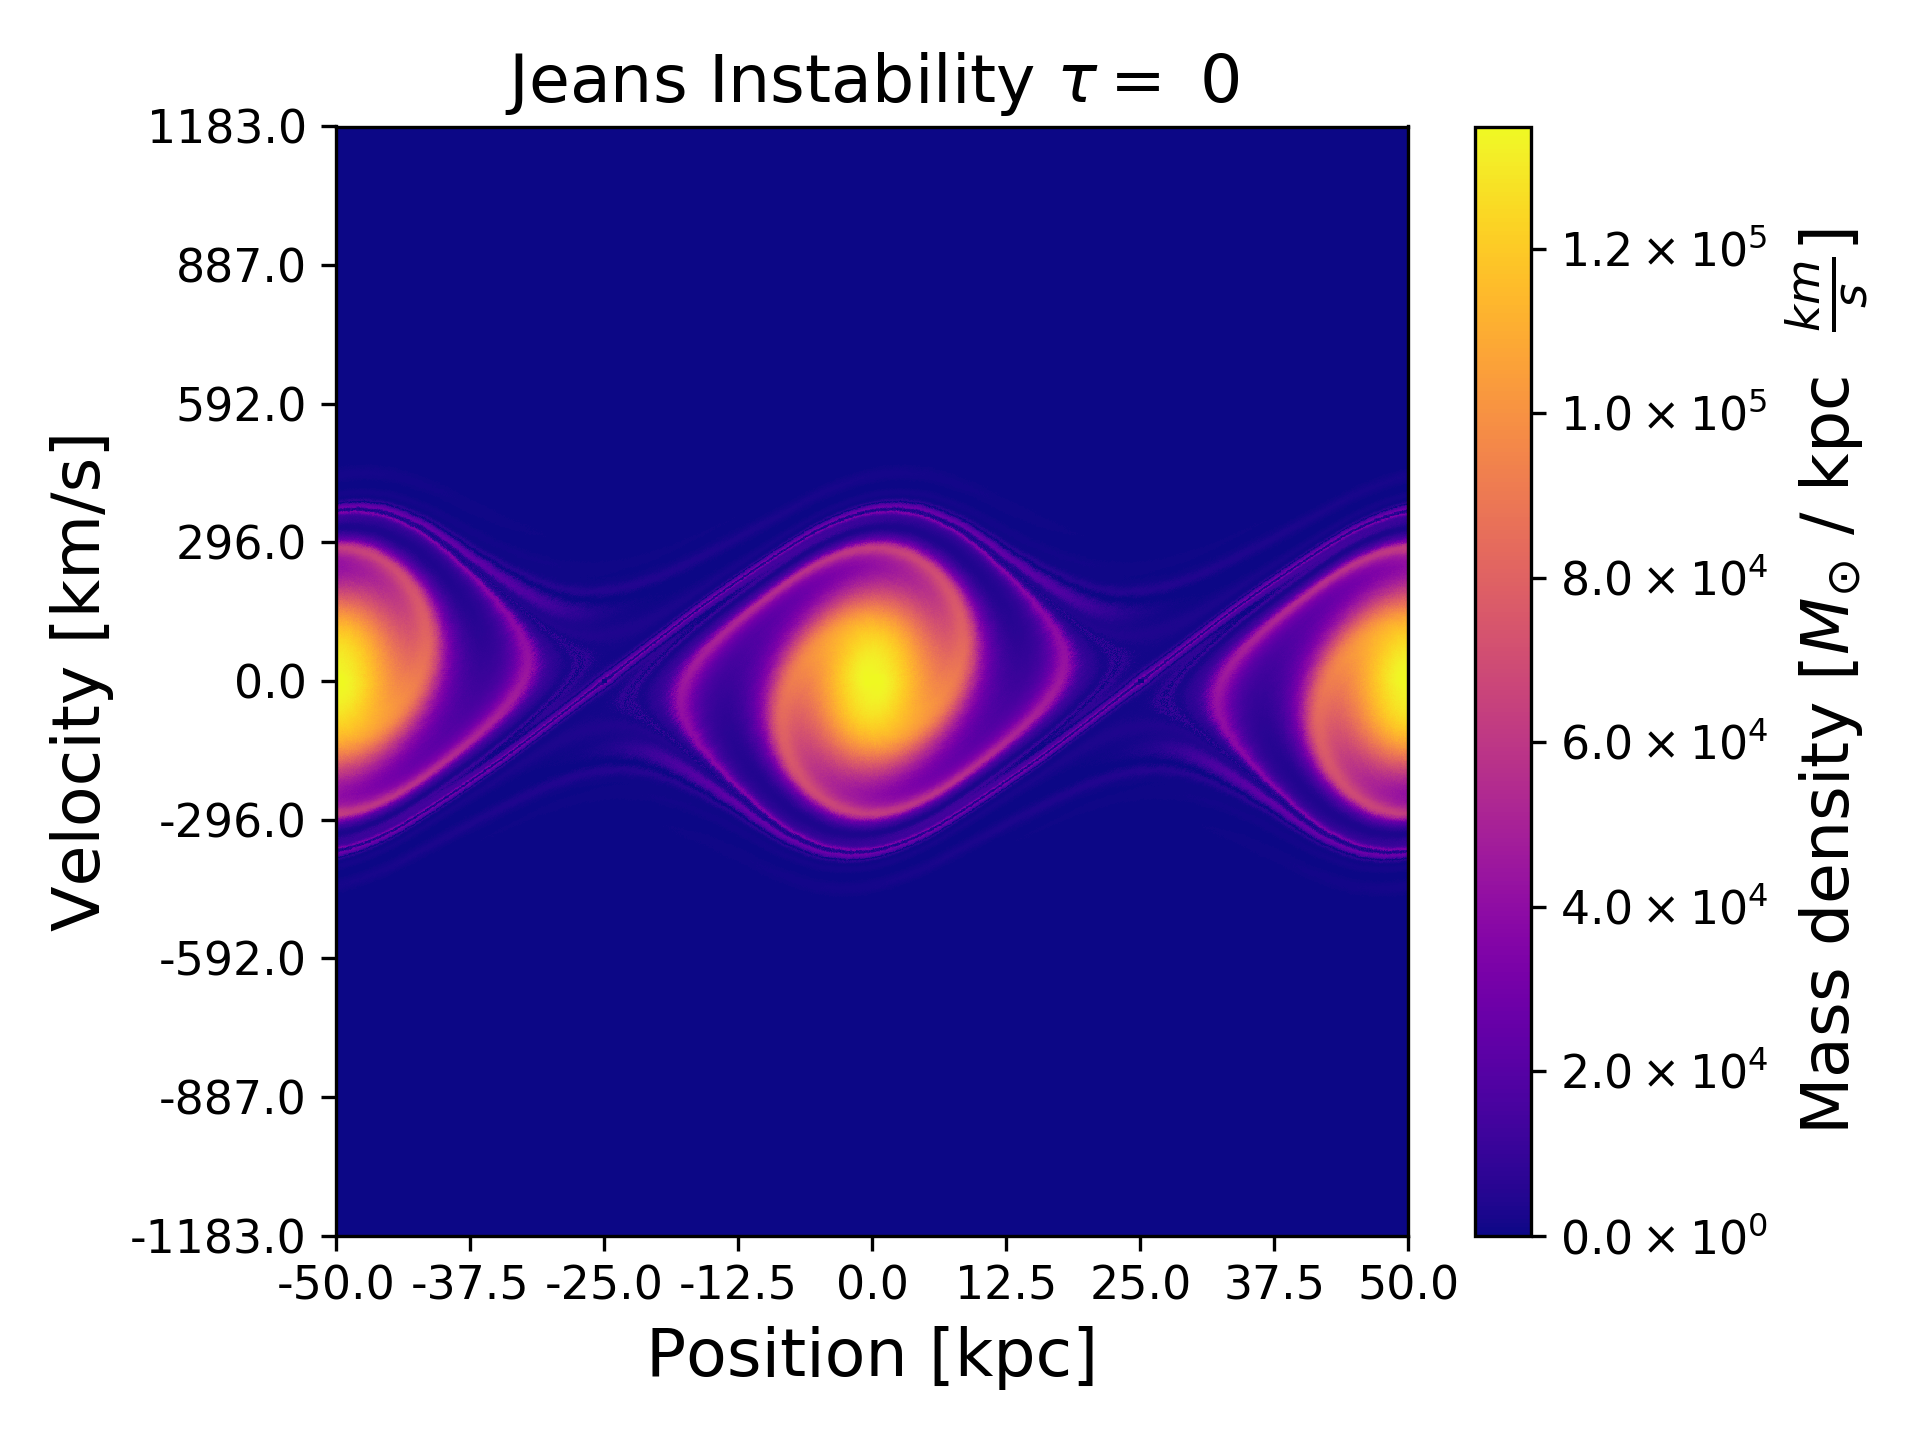
\includegraphics[scale=0.45]{imag/jeans40.png}
    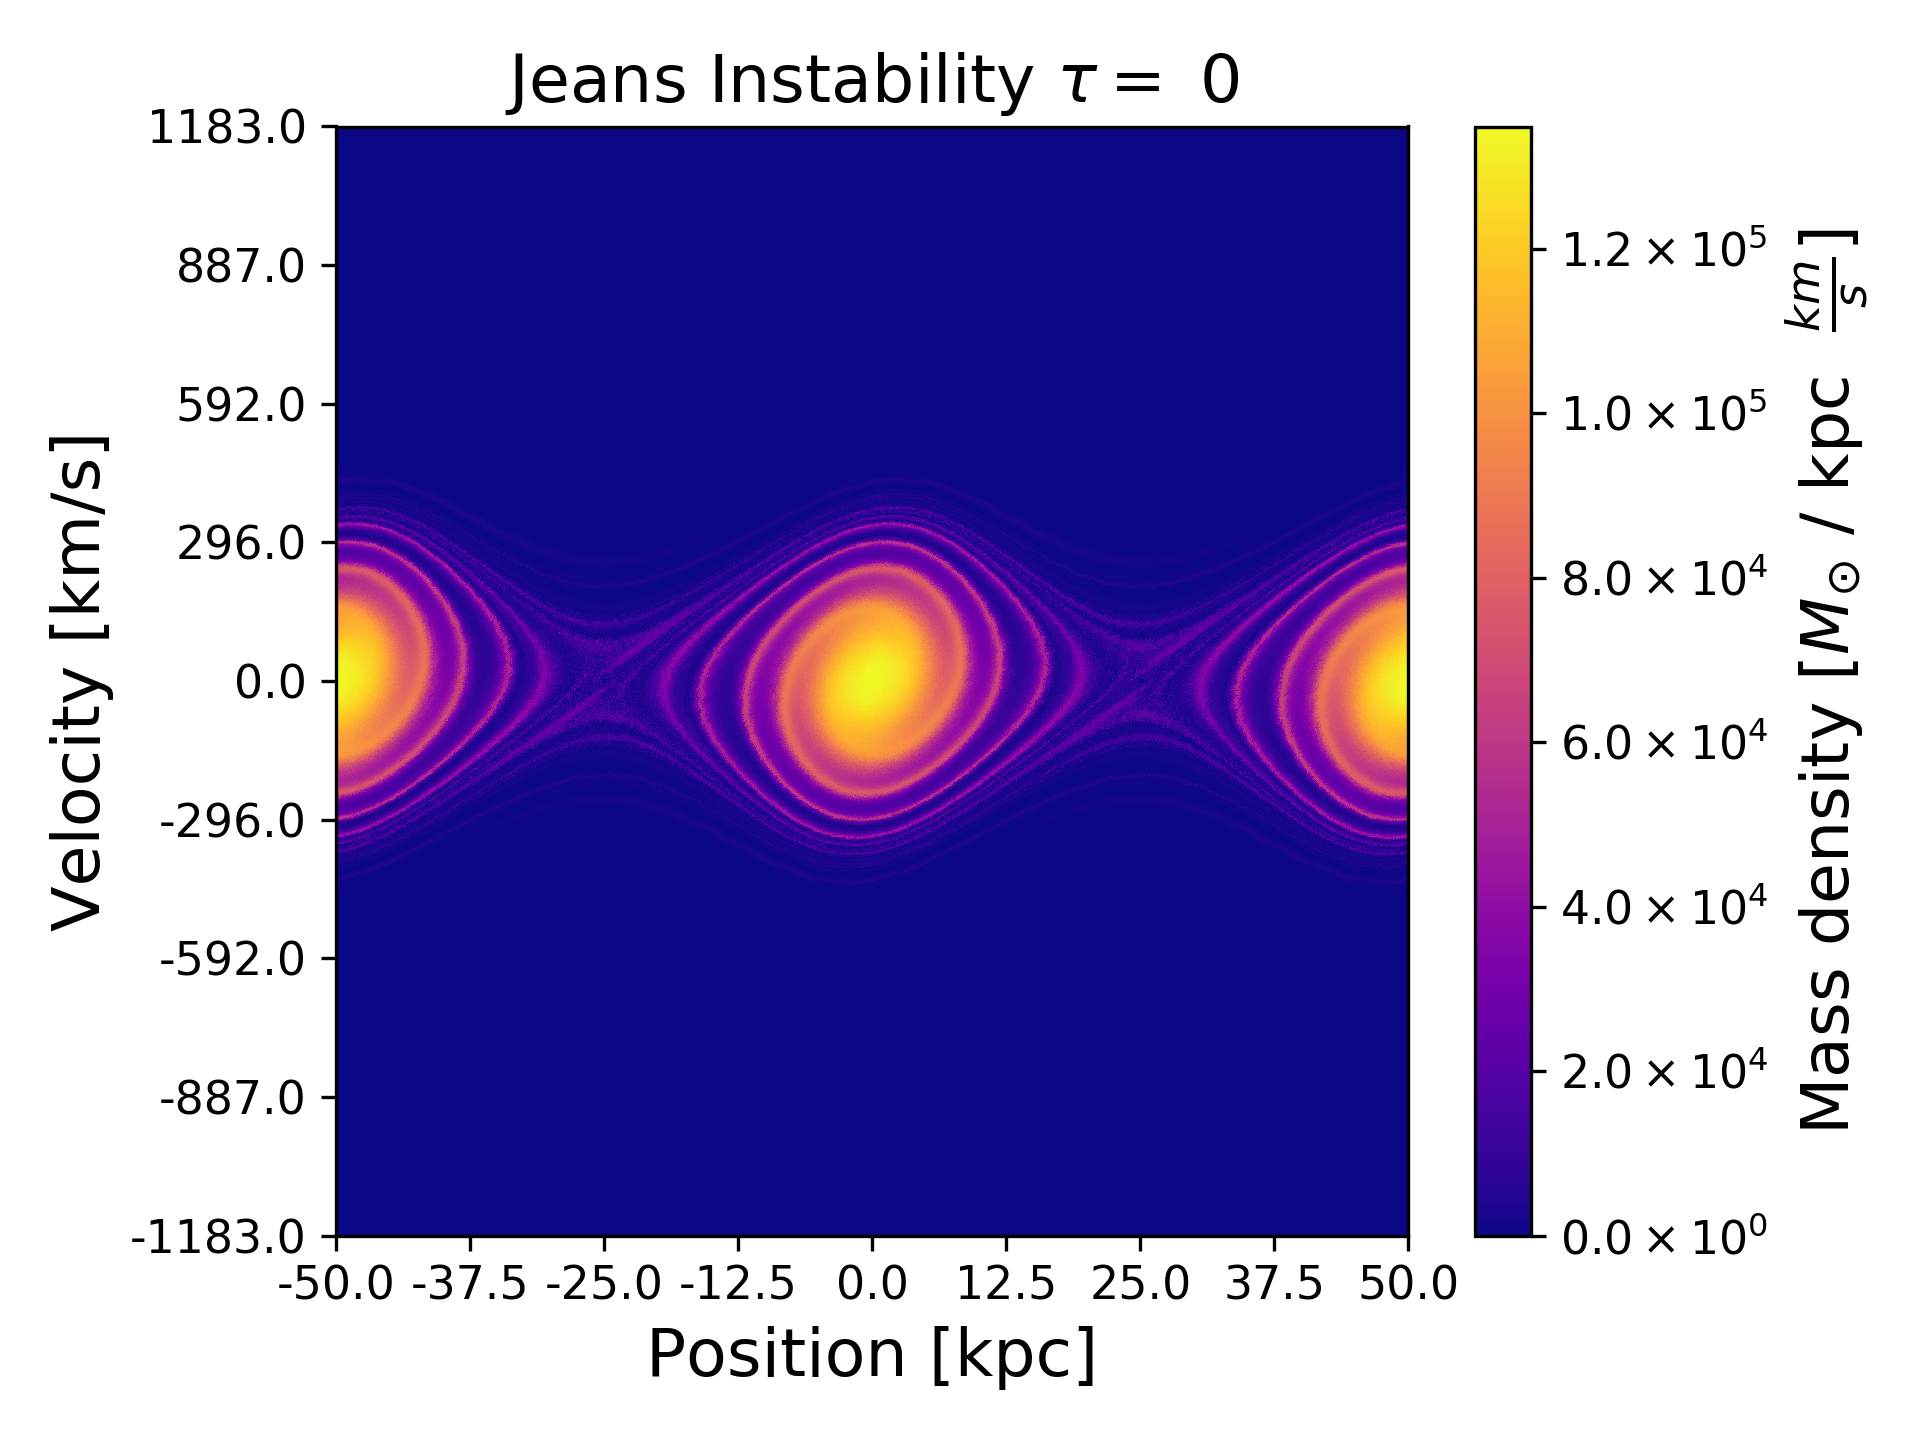
\includegraphics[scale=0.45]{imag/jeans90.png}
    \caption{Upper left: Phase space 72 million years after initialization. Upper right: Phase space 227 million years after initialization. Bottom left: Phase space 413 million years after initialization. Bottom right: Phase space 930 million years after initialization. The behavior is the same as three successive Gaussian conditions.}
    \label{1dJeans}
\end{figure}


\newpage
\section{Four dimensional phase space}
In the case of the four dimensional phase space we need four axes to describe the phase space. This increase in the number of axes in regards to the two dimensional case means that we are going to have to sacrifice a lot of resolution in order to comply to RAM memory constrains. The four dimensional grid used is characterized by:
\begin{align}
W_{min} &= -1\\
W_{max} &= 1\\
N_w &= 128\\
dw &= 1/64
\end{align}
Likewise, the of units to use are:
\begin{align}
1\ us &= 50\ \text{kpc}\\
1\ ut &= 0.003 \ \text{t}_0\\
1\ um &= 10^{11} \ \text{M}_{\astrosun}
\end{align}
With t$_0$ being the age of the universe today, \text{M}$_{\astrosun}$ being a solar mass and a kiloparsec (kpc) is equal to $3.0857\e{19}$ m. In this units, the gravitational constant has a value of:
\begin{equation}
G = 0.006141 \ (1 \ us)^3 \ (1 \ um)^{-1} \ (1 \ ut)^{-2}
\end{equation}
\subsection{No collisional case}
The four dimensional case is initialized using a Gaussian distribution.














\newpage
\section{Six dimensional phase space}
%\section{No collisional}
%\section{Collisional with reported $<\sigma v>$}
%\section{Different equlibrium distributions}










